\chapter{Code as data, data as code}\label{codeanddatachap}

\begin{objectives} \label[objectives]{See-one-of-the-most-impor}

\begin{itemize}
\tightlist
\item
  See one of the most important concepts in computing: duality between
  code and data.\\
\item
  Build up comfort in moving between different representations of
  programs.\\
\item
  Follow the construction of a ``universal circuit evaluator'' that can
  evaluate other circuits given their representation.\\
\item
  See major result that complements the result of the last chapter: some
  functions require an \emph{exponential} number of gates to compute.
\item
  Discussion of \emph{Physical extended Church-Turing thesis} stating
  that Boolean circuits capture \emph{all} feasible computation in the
  physical world, and its physical and philosophical implications.
\end{itemize}

\end{objectives}

\begin{quote}
\emph{``The term code script is, of course, too narrow. The chromosomal
structures are at the same time instrumental in bringing about the
development they foreshadow. They are law-code and executive power - or,
to use another simile, they are architect's plan and builder's craft -
in one.''} , Erwin Schrödinger, 1944.
\end{quote}

\begin{quote}
\emph{``A mathematician would hardly call a correspondence between the
set of 64 triples of four units and a set of twenty other
units,''universal``, while such correspondence is, probably, the most
fundamental general feature of life on Earth''}, Misha Gromov, 2013
\end{quote}

A program is simply a sequence of symbols, each of which can be encoded
as a string of \(0\)'s and \(1\)'s using (for example) the ASCII
standard. Therefore we can represent every NAND-CIRC program (and hence
also every Boolean circuit) as a binary string. This statement seems
obvious but it is actually quite profound. It means that we can treat
circuits or NAND-CIRC programs both as instructions to carrying
computation and also as \emph{data} that could potentially be used as
\emph{inputs} to other computations.

\hypertarget{programisinput}{}
\begin{bigidea} \label[bigidea]{programisinput}

A \emph{program} is a piece of text, and so it can be fed as input to
other programs.

\end{bigidea}

This correspondence between \emph{code} and \emph{data} is one of the
most fundamental aspects of computing. It underlies the notion of
\emph{general purpose} computers, that are not pre-wired to compute only
one task, and also forms the basis of our hope for obtaining
\emph{general} artificial intelligence. This concept finds immense use
in all areas of computing, from scripting languages to machine learning,
but it is fair to say that we haven't yet fully mastered it. Many
security exploits involve cases such as ``buffer overflows'' when
attackers manage to inject code where the system expected only
``passive'' data (see \cref{XKCDmomexploitsfig}). The relation between
code and data reaches beyond the realm of electronic computers. For
example, DNA can be thought of as both a program and data (in the words
of Schrödinger, who wrote before the discovery of DNA's structure a book
that inspired Watson and Crick, DNA is both ``architect's plan and
builder's craft'').


\begin{marginfigure}
\centering
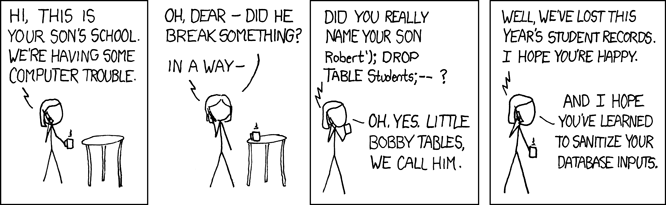
\includegraphics[width=\linewidth, height=1.5in, keepaspectratio]{../figure/exploits_of_a_mom.png}
\caption{As illustrated in this xkcd cartoon, many exploits, including
buffer overflow, SQL injections, and more, utilize the blurry line
between ``active programs'' and ``static strings''.}
\label{XKCDmomexploitsfig}
\end{marginfigure}

In this chapter, we will begin to explore some of the applications of
this connection. We start by using the representation of
programs/circuits as strings to \emph{count} the number of
programs/circuits up to a certain size, and use that to obtain a
counterpart to the result we proved in \cref{finiteuniversalchap}. There
we proved that for \emph{every} function
\(f:\{0,1\}^n \rightarrow \{0,1\}\), there exists a circuit of \emph{at
most} \(100 \cdot 2^n / n\) gates to compute it. (The number \(100\)
here is somewhat arbitrary and fixed for concreteness;
\cref{circuit-univ-thm-improved} states a bound of \(c \cdot 2^n /n\)
for some constant \(c\), but it can be verified that the proof yields
\(c \leq 100\).) In this chapter we will prove that there are
\emph{some} functions \(f:\{0,1\}^n \rightarrow \{0,1\}\) for which we
cannot do much better: they require a circuit of size \emph{at least}
\(0.01 \cdot 2^n / n\) (see \cref{counting-lb}). We will also use the
notion of representing programs/circuits as strings to show the
existence of a \emph{bounded universal circuit} \(U\) that gets as input
the string representation of another circuit \(C\) and a string \(x\),
and outputs \(C(x)\). (The qualifier ``bounded'' means that the circuit
\(C\) has to be of at most a certain size; we see computational models
that overcome this limitation in \cref{chaploops}, which introduces the
notion of programming languages with \emph{loops} and the computational
model of a \emph{Turing Machine}.) Equivalently, taking the
programming-language point of view, the bounded universal circuit
corresponds to a ``NAND-CIRC interpreter in NAND-CIRC'': a NAND-CIRC
program that can evaluate other NAND-CIRC program. Such a program is
known in Computer Science as a ``meta-circular evaluator'', and is
fundamental to both theory and practice of computing. See
\cref{codedataoverviewfig} for an overview of the results of this
chapter.


\begin{figure}
\centering
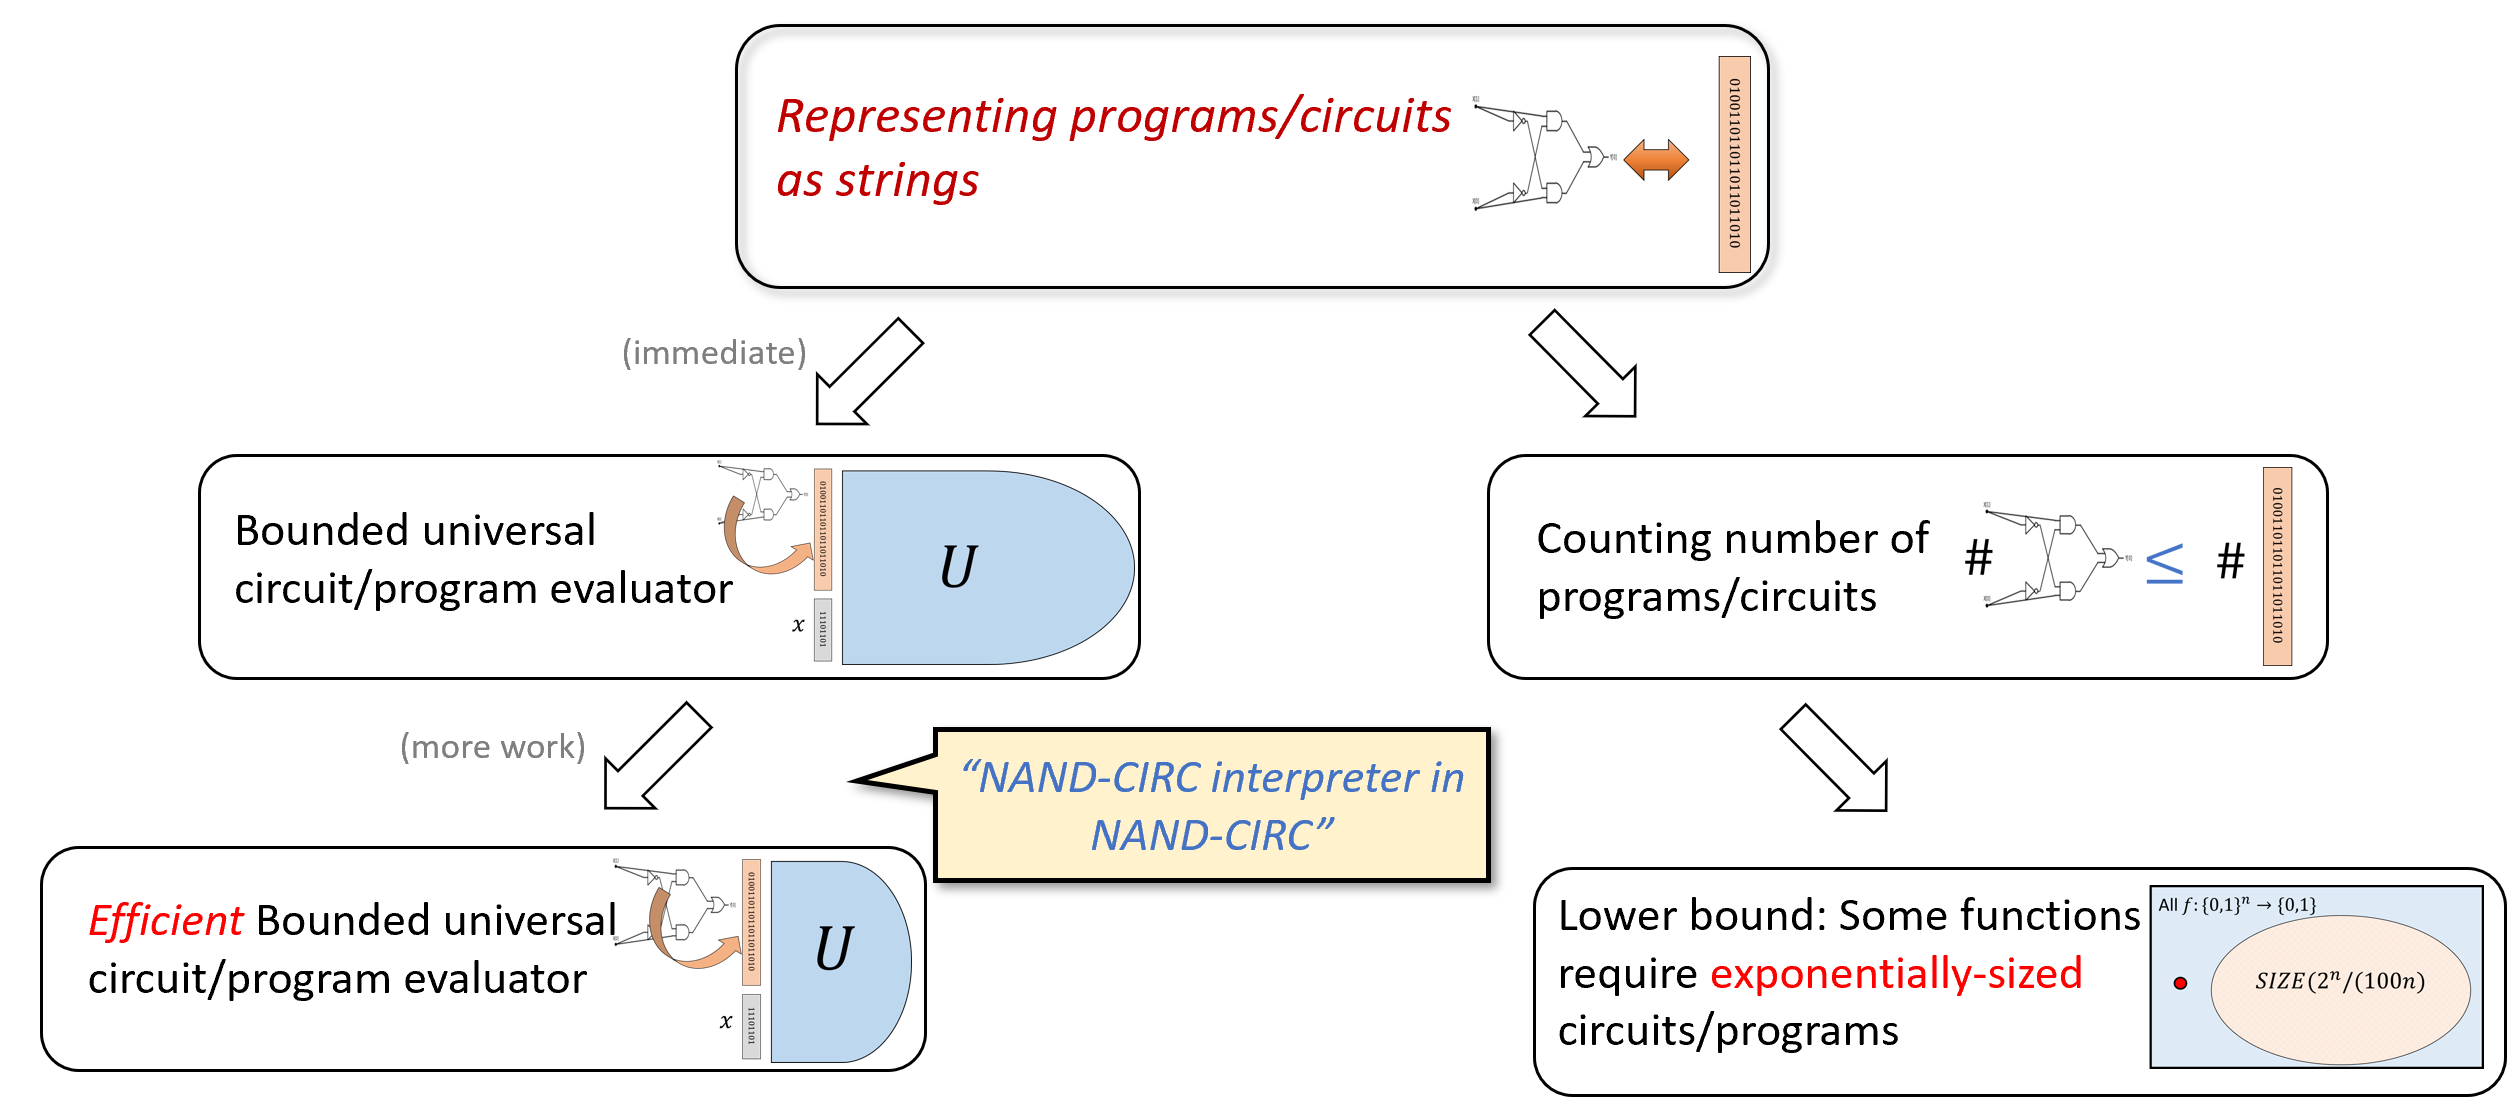
\includegraphics[width=\textwidth, height=0.25\paperheight, keepaspectratio]{../figure/codedataoverview.png}
\caption{Overview of the results in this chapter. We use the
representation of programs/circuits as strings to derive two main
results. First we show the existence of a universal program/circuit, and
in fact (with more work) the existence of such a program/circuit whose
size is at most polynomial in the size of the program/circuit it
evaluates. We then use the string representation to \emph{count} the
number of programs/circuits of a given size, and use that to establish
that \emph{some} functions require an \emph{exponential} number of
lines/gates to compute.}
\label{codedataoverviewfig}
\end{figure}

\section{Representing programs as strings}\label{representprogramsec}


\begin{marginfigure}
\centering
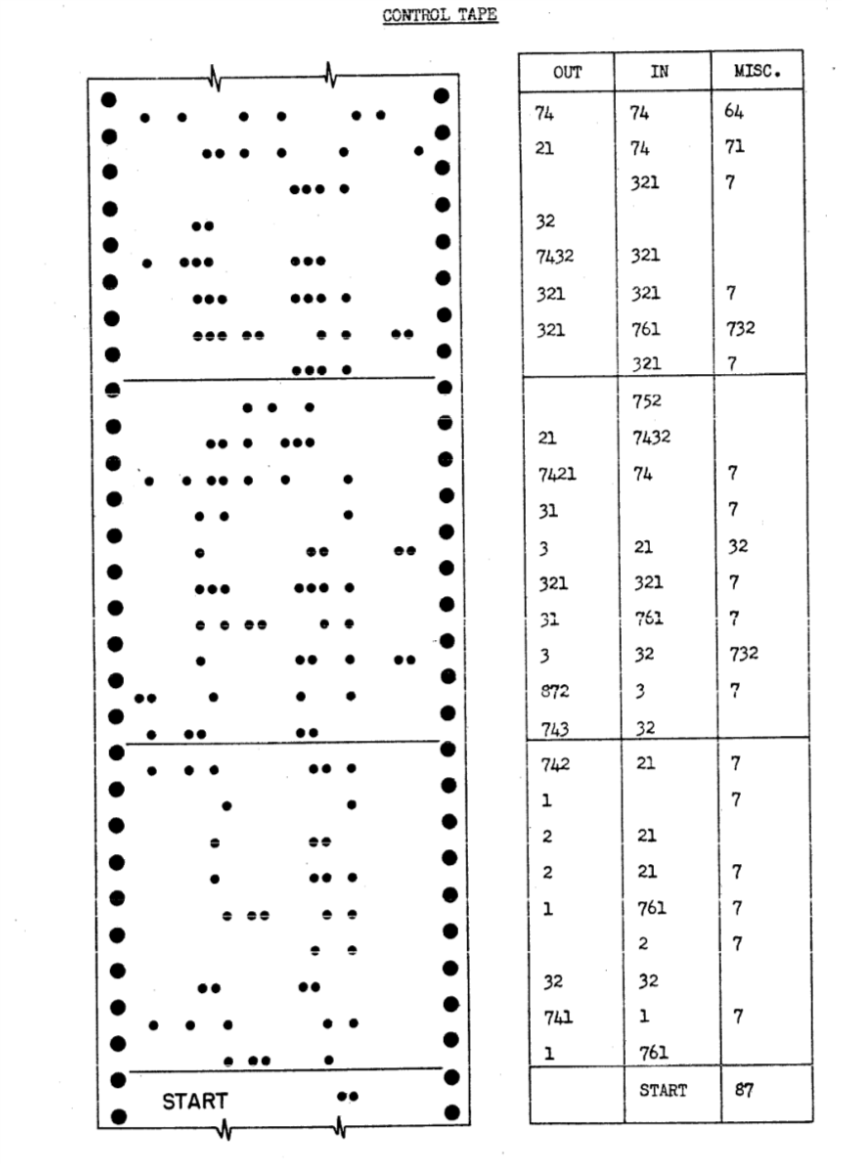
\includegraphics[width=\linewidth, height=1.5in, keepaspectratio]{../figure/tapemarkI.png}
\caption{In the Harvard Mark I computer, a program was represented as a
list of triples of numbers, which were then encoded by perforating holes
in a control card.}
\label{markonerep}
\end{marginfigure}

We can represent programs or circuits as strings in a myriad of ways.
For example, since Boolean circuits are labeled directed acyclic graphs,
we can use the \emph{adjacency matrix} or \emph{adjacency list}
representations for them. However, since the code of a program is
ultimately just a sequence of letters and symbols, arguably the
conceptually simplest representation of a program is as such a sequence.
For example, the following NAND-CIRC program \(P\)

\begin{code}
temp_0 = NAND(X[0],X[1])
temp_1 = NAND(X[0],temp_0)
temp_2 = NAND(X[1],temp_0)
Y[0] = NAND(temp_1,temp_2)
\end{code}

is simply a string of 107 symbols which include lower and upper case
letters, digits, the underscore character \texttt{\_} and equality sign
\texttt{=}, punctuation marks such as
``\texttt{(}'',``\texttt{)}'',``\texttt{,}'', spaces, and ``new line''
markers (often denoted as ``\texttt{\textbackslash n}'' or ``↵''). Each
such symbol can be encoded as a string of \(7\) bits using the
\href{https://en.wikipedia.org/wiki/ASCII}{ASCII} encoding, and hence
the program \(P\) can be encoded as a string of length
\(7 \cdot 107 = 749\) bits.

Nothing in the above discussion was specific to the program \(P\), and
hence we can use the same reasoning to prove that \emph{every} NAND-CIRC
program can be represented as a string in \(\{0,1\}^*\). In fact, we can
do a bit better. Since the names of the working variables of a NAND-CIRC
program do not affect its functionality, we can always transform a
program to have the form of \(P'\) where all variables apart from the
inputs and outputs have the form \texttt{temp\_0}, \texttt{temp\_1},
\texttt{temp\_2}, etc.. Moreover, if the program has \(s\) lines, then
we will never need to use an index larger than \(3s\) (since each line
involves at most three variables), and similarly the indices of the
input and output variables will all be at most \(3s\). Since a number
between \(0\) and \(3s\) can be expressed using at most
\(\lceil \log_{10}(3s+1) \rceil = O(\log s)\) digits, each line in the
program (which has the form \texttt{foo = NAND(bar,blah)}), can be
represented using \(O(1) + O(\log s) = O(\log s)\) symbols, each of
which can be represented by \(7\) bits. Hence an \(s\) line program can
be represented as a string of \(O(s \log s)\) bits, resulting in the
following theorem:

\hypertarget{asciirepprogramthm}{}
\begin{theorem}[Representing programs as strings] \label[theorem]{asciirepprogramthm}

There is a constant \(c\) such that for
\(f \in \ensuremath{\mathit{SIZE}}(s)\), there exists a program \(P\)
computing \(f\) whose string representation has length at most
\(c s \log s\).

\end{theorem}

\begin{pause} \label[pause]{We-omit-the-formal-proof-}

We omit the formal proof of \cref{asciirepprogramthm} but please make
sure that you understand why it follows from the reasoning above.

\end{pause}

\section{Counting programs, and lower bounds on the size of NAND-CIRC
programs}\label{countingcircuitsec}

One consequence of the representation of programs as strings is that the
number of programs of certain length is bounded by the number of strings
that represent them. This has consequences for the sets
\(\ensuremath{\mathit{SIZE}}(s)\) that we defined in
\cref{secdefinesizeclasses}.

\hypertarget{program-count}{}
\begin{theorem}[Counting programs] \label[theorem]{program-count}

For every \(s\in \N\),
\[|\ensuremath{\mathit{SIZE}}(s)| \leq 2^{O(s \log s)}.\] That is, there
are at most \(2^{O(s\log s)}\) functions computed by NAND-CIRC programs
of at most \(s\) lines.\footnote{The implicit constant in the
  \(O(\cdot)\) notation is smaller than \(10\). That is, for all
  sufficiently large \(s\),
  \(|\ensuremath{\mathit{SIZE}}(s)|< 2^{10s\log s}\), see
  \cref{efficientrepresentation}. As discussed in \cref{notationsec}, we
  use the bound \(10\) simply because it is a round number.}

\end{theorem}

\begin{proof} \label[proof]{We-will-show-a-one-to-one}

We will show a one-to-one map \(E\) from
\(\ensuremath{\mathit{SIZE}}(s)\) to the set of strings of length
\(c s \log s\) for some constant \(c\). This will conclude the proof,
since it implies that \(|\ensuremath{\mathit{SIZE}}(s)|\) is smaller
than the size of the set of all strings of length at most \(\ell\),
which equals \(1+2+4+\cdots + 2^\ell = 2^{\ell +1} - 1\) by the formula
for sums of geometric progressions.

The map \(E\) will simply map \(f\) to the representation of the program
computing \(f\). Specifically, we let \(E(f)\) be the representation of
the program \(P\) computing \(f\) given by \cref{asciirepprogramthm}.
This representation has size at most \(c s \log s\), and moreover the
map \(E\) is one to one, since if \(f \neq f'\) then every two programs
computing \(f\) and \(f'\) respectively must have different
representations.

\end{proof}

A function mapping \(\{0,1\}^2\) to \(\{0,1\}\) can be identified with
the table of its four values on the inputs \(00,01,10,11\). A function
mapping \(\{0,1\}^3\) to \(\{0,1\}\) can be identified with the table of
its eight values on the inputs \(000,001,010,011,100,101,110,111\). More
generally, every function \(F:\{0,1\}^n \rightarrow \{0,1\}\) can be
identified with the table of its \(2^n\) values on the inputs
\(\{0,1\}^n\). Hence the number of functions mapping \(\{0,1\}^n\) to
\(\{0,1\}\) is equal to the number of such tables which (since we can
choose either \(0\) or \(1\) for every row) is exactly \(2^{2^n}\). Note
that this is \emph{double exponential} in \(n\), and hence even for
small values of \(n\) (e.g., \(n=10\)) the number of functions from
\(\{0,1\}^n\) to \(\{0,1\}\) is truly astronomical.\footnote{``Astronomical''
  here is an understatement: there are much fewer than \(2^{2^{10}}\)
  stars, or even particles, in the observable universe.} This has the
following important corollary:

\hypertarget{counting-lb}{}
\begin{theorem}[Counting argument lower bound] \label[theorem]{counting-lb}

There is a constant \(\delta > 0\), such that for every sufficiently
large \(n\), there is a function \(f:\{0,1\}^n\rightarrow \{0,1\}\) such
that
\(f \not\in \ensuremath{\mathit{SIZE}} \left(\tfrac{\delta 2^n}{n} \right)\).
That is, the shortest NAND-CIRC program to compute \(F\) requires at
least \(\delta \cdot 2^n/n\) lines.\footnote{The constant \(\delta\) is
  at least \(0.1\) and in fact, can be improved to be arbitrarily close
  to \(1/2\), see \cref{efficientlbex}.}

\end{theorem}

\begin{proof} \label[proof]{The-proof-is-simple-If-we}

The proof is simple. If we let \(c\) be the constant such that
\(|\ensuremath{\mathit{SIZE}}(s)| \leq 2^{c s \log s}\) and
\(\delta = 1/c\), then setting \(s = \delta 2^n/n\) we see that \[
|\ensuremath{\mathit{SIZE}}(\tfrac{\delta 2^n}{n})| \leq 2^{c \tfrac{\delta 2^n}{n} \log s} < 2^{c \delta 2^n} = 2^{2^n}
\] using the fact that since \(s < 2^n\), \(\log s < n\) and
\(\delta = 1/c\). But since \(|\ensuremath{\mathit{SIZE}}(s)|\) is
smaller than the total number of functions mapping \(n\) bits to \(1\)
bit, there must be at least one such function not in
\(\ensuremath{\mathit{SIZE}}(s)\), which is what we needed to prove.

\end{proof}

We have seen before that \emph{every} function mapping \(\{0,1\}^n\) to
\(\{0,1\}\) can be computed by an \(O(2^n /n)\) line program.
\cref{counting-lb} shows that this is tight in the sense that some
functions do require such an astronomical number of lines to compute.

\hypertarget{countinglb}{}
\begin{bigidea} \label[bigidea]{countinglb}

Some functions \(f:\{0,1\}^n \rightarrow \{0,1\}\) \emph{cannot} be
computed by a Boolean circuit using fewer than exponential (in \(n\))
number of gates.

\end{bigidea}

In fact, as we explore in the exercises, this is the case for
\emph{most} functions. Hence functions that can be computed in a small
number of lines (such as addition, multiplication, finding short paths
in graphs, or even the \(\ensuremath{\mathit{EVAL}}\) function) are the
exception, rather than the rule.

\hypertarget{efficientrepresentation}{}
\begin{remark}[More efficient representation (advanced, optional)] \label[remark]{efficientrepresentation}

The ASCII representation is not the shortest representation for
NAND-CIRC programs. NAND-CIRC programs are equivalent to circuits with
NAND gates, which means that a NAND-CIRC program of \(s\) lines, \(n\)
inputs, and \(m\) outputs can be represented by a labeled directed graph
of \(s+n\) vertices, of which \(n\) have in-degree zero, and the \(s\)
others have in-degree at most two. Using the adjacency matrix
representation for such graphs, we can reduce the implicit constant in
\cref{program-count} to be arbitrarily close to \(5\), see
\cref{efficientrepresentationex}

\end{remark}

\subsection{Size hierarchy theorem
(optional)}\label{Size-hierarchy-theorem-op}

By \cref{NAND-univ-thm-improved} the class
\(\ensuremath{\mathit{SIZE}}_{n}(10 \cdot 2^n /n)\) contains \emph{all}
functions from \(\{0,1\}^n\) to \(\{0,1\}\), while by
\cref{counting-lb}, there is \emph{some} function
\(f:\{0,1\}^n \rightarrow \{0,1\}\) that is \emph{not contained} in
\(\ensuremath{\mathit{SIZE}}_{n}(0.1 \cdot 2^n / n)\). In other words,
for every sufficiently large \(n\), \[
\ensuremath{\mathit{SIZE}}_n\left(0.1 \tfrac{2^n}{n} \right) \subsetneq \ensuremath{\mathit{SIZE}}_n\left(10 \tfrac{2^n}{n} \right) \;.
\] It turns out that we can use \cref{counting-lb} to show a more
general result: whenever we increase our ``budget'' of gates we can
compute new functions.

\hypertarget{sizehiearchythm}{}
\begin{theorem}[Size Hierarchy Theorem] \label[theorem]{sizehiearchythm}

For every sufficiently large \(n\) and \(10n < s < 0.1 \cdot 2^n /n\),
\[
\ensuremath{\mathit{SIZE}}_n(s) \subsetneq \ensuremath{\mathit{SIZE}}_n(s+10n) \;.
\]

\end{theorem}

\begin{proofidea} \label[proofidea]{To-prove-the-theorem-we-n}

To prove the theorem we need to find a function
\(f:\{0,1\}^n \rightarrow \{0,1\}\) such that \(f\) \emph{can} be
computed by a circuit of \(s+10n\) gates but it \emph{cannot} be
computed by a circuit of \(s\) gates. We will do so by coming up with a
sequence of functions \(f_0,f_1,f_2,\ldots,f_N\) with the following
properties: \textbf{(1)} \(f_0\) \emph{can} be computed by a circuit of
at most \(10n\) gates, \textbf{(2)} \(f_N\) \emph{cannot} be computed by
a circuit of \(0.1 \cdot 2^n/n\) gates, and \textbf{(3)} for every
\(i\in \{0,\ldots, N\}\), if \(f_i\) can be computed by a circuit of
size \(s\), then \(f_{i+1}\) can be computed by a circuit of size at
most \(s + 10n\). Together these properties imply that if we let \(i\)
be the smallest number such that
\(f_i \not\in \ensuremath{\mathit{SIZE}}_n(s)\), then since
\(f_{i+1} \in \ensuremath{\mathit{SIZE}}(s)\) it must hold that
\(f_i \in \ensuremath{\mathit{SIZE}}(s+10n)\) which is what we need to
prove. See \cref{hierarchyprooffig} for an illustration.

\end{proofidea}


\begin{marginfigure}
\centering
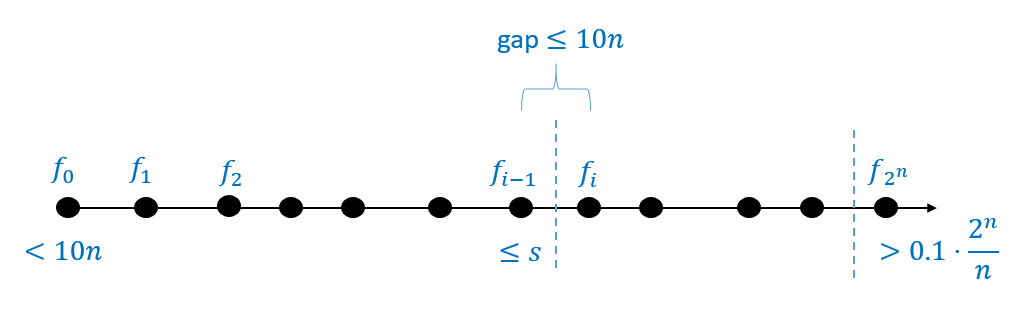
\includegraphics[width=\linewidth, height=1.5in, keepaspectratio]{../figure/hierarchyproof.png}
\caption{We prove \cref{sizehiearchythm} by coming up with a list
\(f_0,\ldots,f_{2^n}\) of functions such that \(f_0\) is the all zero
function, \(f_{2^n}\) is a function (obtained from \cref{counting-lb})
outside of \(\ensuremath{\mathit{SIZE}}(0.1\cdot 2^n/n)\) and such that
\(f_{i-1}\) and \(f_i\) differ by one another on at most one input. We
can show that for every \(i\), the number of gates to compute \(f_i\) is
at most \(10n\) larger than the number of gates to compute \(f_{i-1}\)
and so if we let \(i\) be the smallest number such that
\(f_i \not\in \ensuremath{\mathit{SIZE}}(s)\), then
\(f_i \in \ensuremath{\mathit{SIZE}}(s+10n)\).}
\label{hierarchyprooffig}
\end{marginfigure}

\begin{proof}[Proof of \cref{sizehiearchythm}] \label[proof]{Let-f-n-rightarrow--be-th}

Let \(f^*: \{0,1\}^n \rightarrow \{0,1\}\) be the function (whose
existence we are guaranteed by \cref{counting-lb}) such that
\(f^* \not\in \ensuremath{\mathit{SIZE}}_n(0.1 \cdot 2^n /n)\). We
define the functions \(f_0,f_1,\ldots, f_{2^n}\) mapping \(\{0,1\}^n\)
to \(\{0,1\}\) as follows. For every \(x\in \{0,1\}^n\), if
\(lex(x) \in \{0,1,\ldots, 2^n-1\}\) is \(x\)'s order in the
lexicographical order then \[
f_i(x) = \begin{cases} f^*(x) & lex(x)< i  \\ 0 & \text{otherwise} \end{cases} \;.
\]

The function \(f_0\) is simply the constant zero function, while the
function \(f_{2^n}\) is equal to \(f^*\). Moreover, for every
\(i\in [2^n]\), the functions \(f_i\) and \(f_{i+1}\) differ on at most
one input (i.e., the input \(x \in \{0,1\}^n\) such that \(lex(x)=i\)).
Let \(10n < s < 0.1 \cdot 2^n /n\), and let \(i\) be the first index
such that \(f_i \not\in \ensuremath{\mathit{SIZE}}_n(s)\). Since
\(f_{2^n} = f^* \not\in \ensuremath{\mathit{SIZE}}(0.1 \dot 2^n / n)\)
there must exist such an index \(i\), and moreover \(i>0\) since the
constant zero function is a member of
\(\ensuremath{\mathit{SIZE}}_n(10n)\).

By our choice of \(i\), \(f_{i-1}\) is a member of
\(\ensuremath{\mathit{SIZE}}_n(s)\). To complete the proof, we need to
show that \(f_i \in \ensuremath{\mathit{SIZE}}_n(s + 10n)\). Let \(x^*\)
be the string such that \(lex(x^*)=i\) \(b\in \{0,1\}\) is the value of
\(f^*(x^*)\). Then we can define \(f_i\) also as follows \[
f_i(x) = \begin{cases} b & x=x^* \\ f_i(x) & x \neq x^*
         \end{cases}
\] or in other words \[
f_i(x) = f_{i-1}(x) \wedge \ensuremath{\mathit{EQUAL}}(x^*,x) \; \vee \;  b \wedge \neg \ensuremath{\mathit{EQUAL}}(x^*,x)
\] where
\(\ensuremath{\mathit{EQUAL}}:\{0,1\}^{2n} \rightarrow \{0,1\}\) is the
function that maps \(x,x' \in \{0,1\}^n\) to \(1\) if they are equal and
to \(0\) otherwise. Since (by our choice of \(i\)), \(f_{i-1}\) can be
computed using at most \(s\) gates and (as can be easily verified) that
\(\ensuremath{\mathit{EQUAL}} \in \ensuremath{\mathit{SIZE}}_n(9n)\), we
can compute \(f_i\) using at most \(s + 9n +O(1) \leq s +10n\) gates
which is what we wanted to prove.

\end{proof}


\begin{figure}
\centering
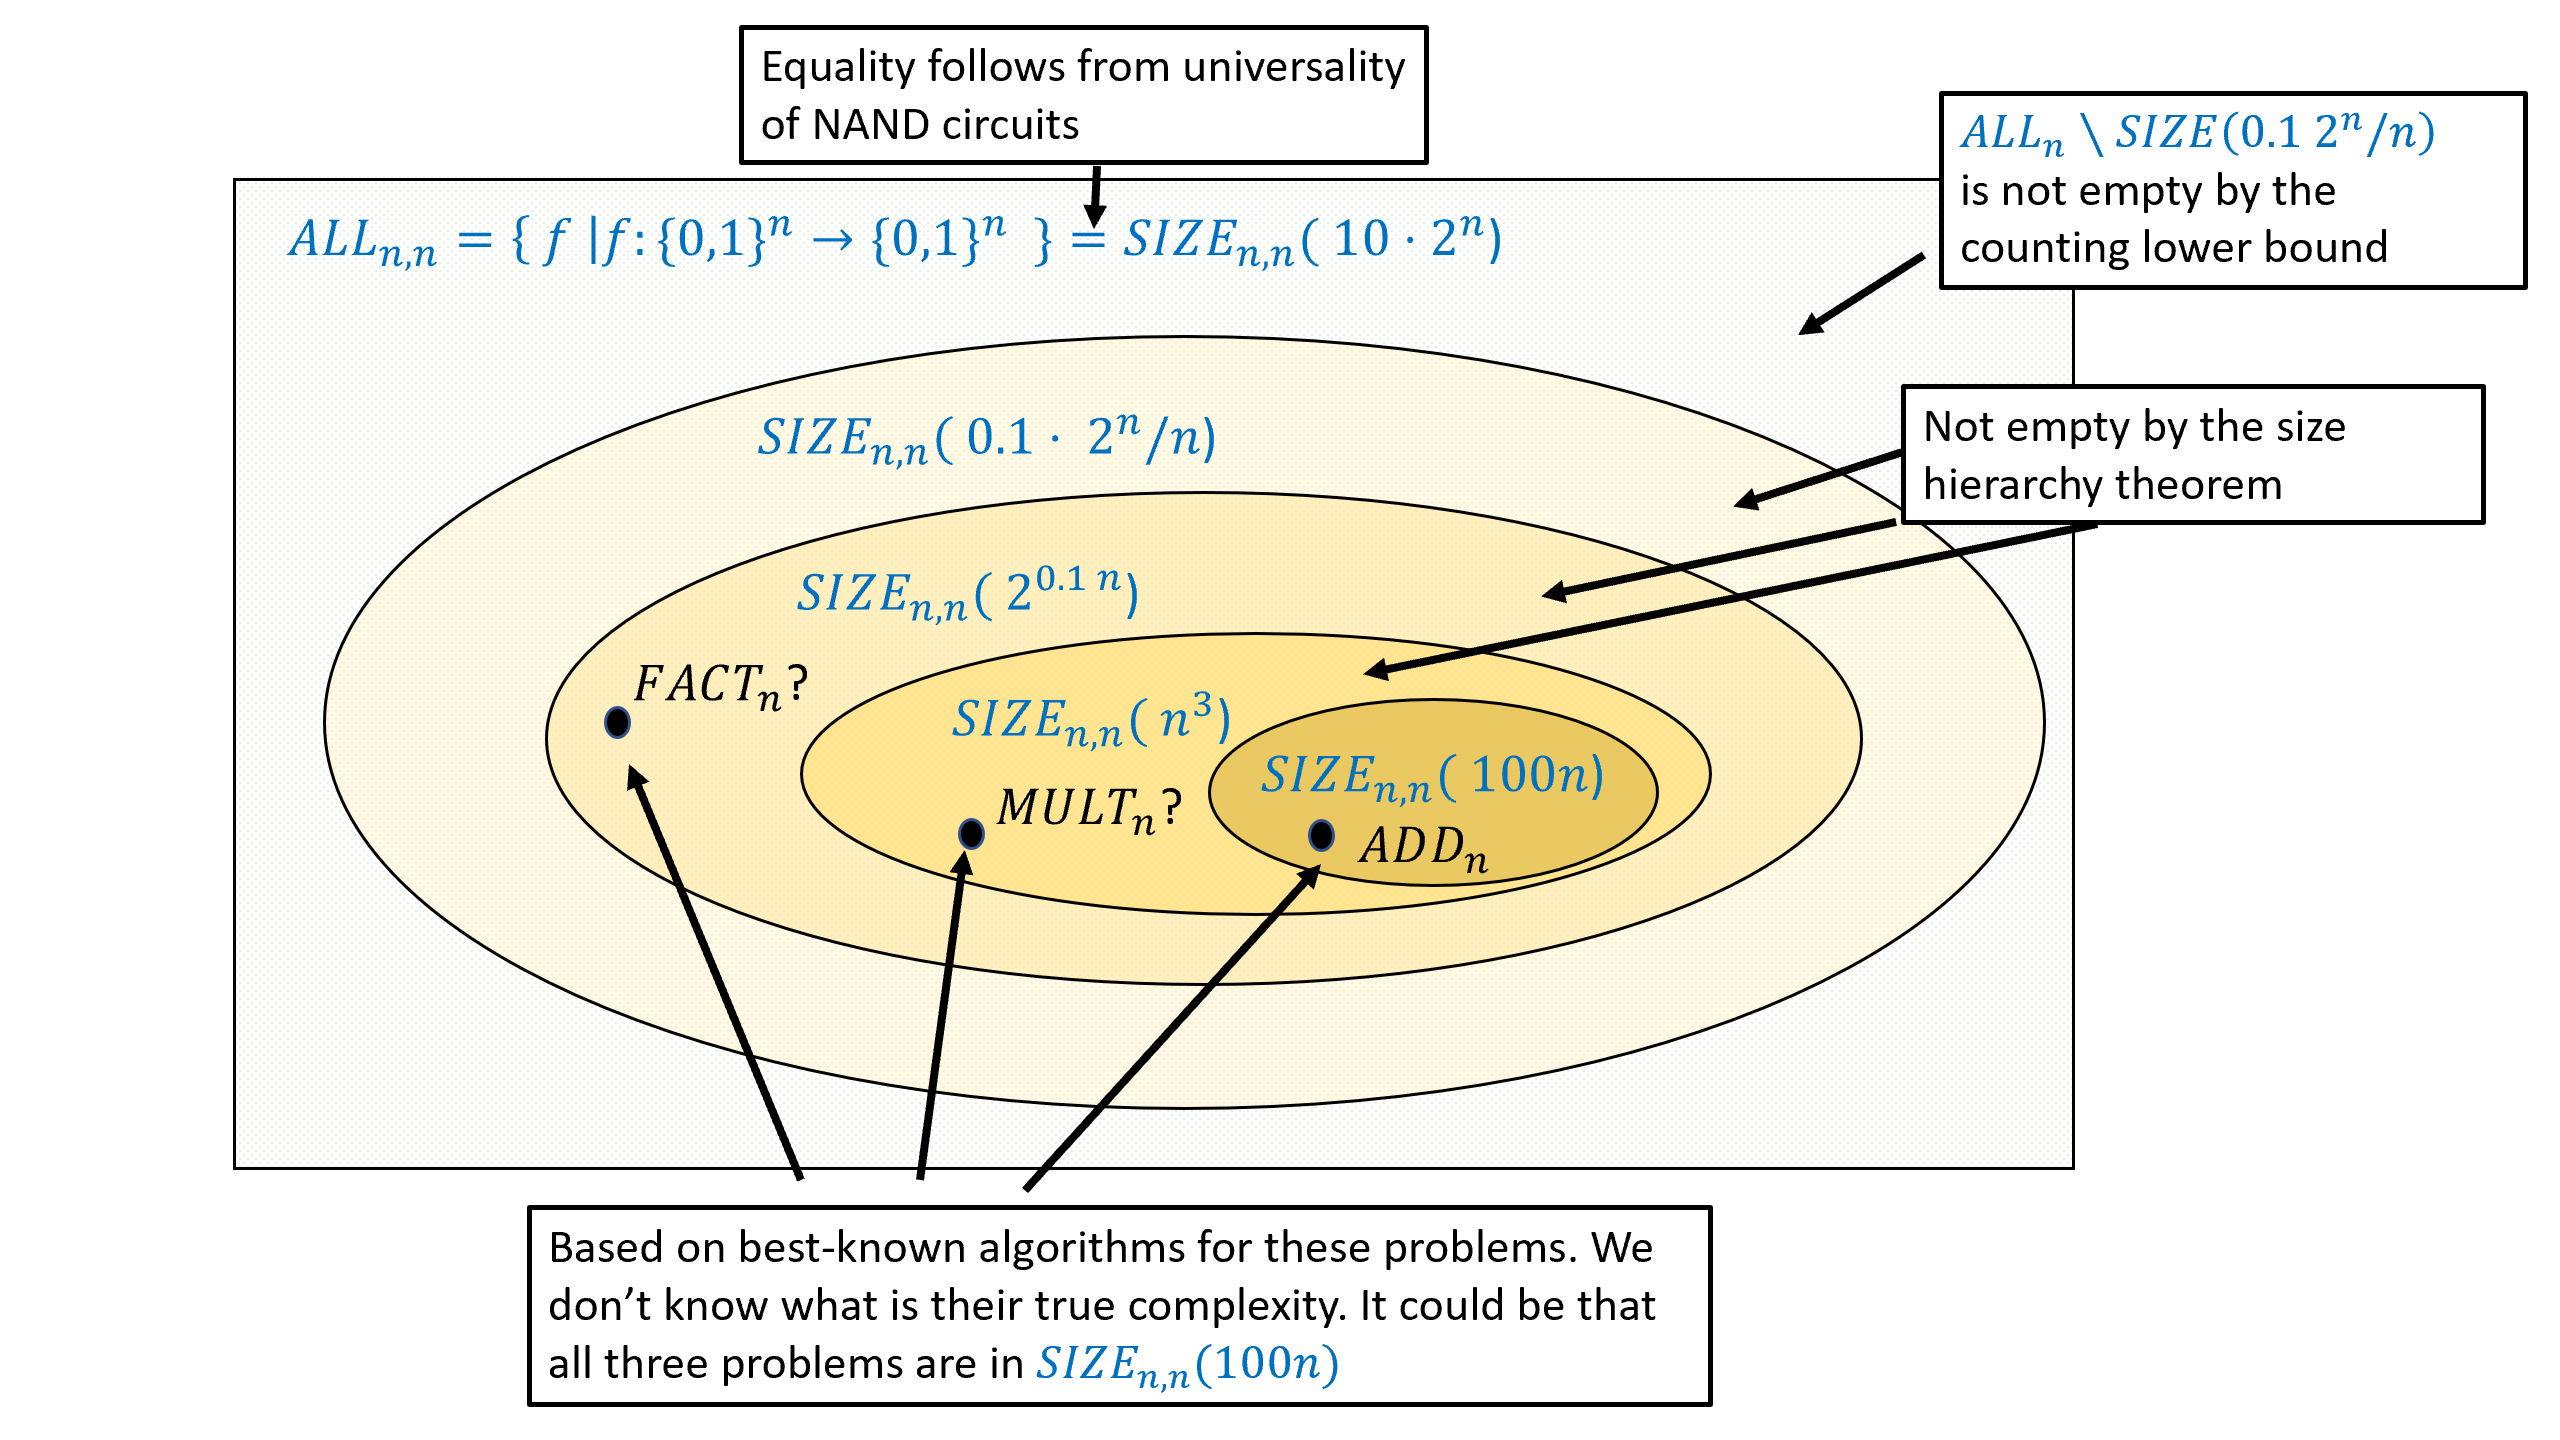
\includegraphics[width=\textwidth, height=0.25\paperheight, keepaspectratio]{../figure/sizecomplexity.png}
\caption{An illustration of some of what we know about the size
complexity classes (not to scale!). This figure depicts classes of the
form \(\ensuremath{\mathit{SIZE}}_{n,n}(s)\) but the state of affairs
for other size complexity classes such as
\(\ensuremath{\mathit{SIZE}}_{n,1}(s)\) is similar. We know by
\cref{NAND-univ-thm} (with the improvement of \cref{tight-upper-bound})
that all functions mapping \(n\) bits to \(n\) bits can be computed by a
circuit of size \(c \cdot 2^n\) for \(c \leq 10\), while on the other
hand the counting lower bound (\cref{counting-lb}, see also
\cref{countingmultibitex}) shows that \emph{some} such functions will
require \(0.1 \cdot 2^n\), and the size hierarchy theorem
(\cref{sizehiearchythm}) shows the existence of functions in
\(\ensuremath{\mathit{SIZE}}(S) \setminus \ensuremath{\mathit{SIZE}}(s)\)
whenever \(s=o(S)\), see also \cref{sizehiearchyex}. We also consider
some specific examples: addition of two \(n/2\) bit numbers can be done
in \(O(n)\) lines, while we don't know of such a program for
\emph{multiplying} two \(n\) bit numbers, though we do know it can be
done in \(O(n^2)\) and in fact even better size. In the above,
\(\ensuremath{\mathit{FACTOR}}_n\) corresponds to the inverse problem of
multiplying- finding the \emph{prime factorization} of a given number.
At the moment we do not know of any circuit a polynomial (or even
sub-exponential) number of lines that can compute
\(\ensuremath{\mathit{FACTOR}}_n\).}
\label{sizeclassesfig}
\end{figure}

\hypertarget{explicitfunc}{}
\begin{remark}[Explicit functions] \label[remark]{explicitfunc}

While the size hierarchy theorem guarantees that there exists
\emph{some} function that \emph{can} be computed using, for example,
\(n^2\) gates, but not using \(100n\) gates, we do not know of any
explicit example of such a function. While we suspect that integer
multiplication is such an example, we do not have any proof that this is
the case.

\end{remark}

\section{The tuples representation}\label{listoftuplesrepsec}

ASCII is a fine presentation of programs, but for some applications it
is useful to have a more concrete representation of NAND-CIRC programs.
In this section we describe a particular choice, that will be convenient
for us later on. A NAND-CIRC program is simply a sequence of lines of
the form

\begin{code}
blah = NAND(baz,boo)
\end{code}

There is of course nothing special about the particular names we use for
variables. Although they would be harder to read, we could write all our
programs using only working variables such as \texttt{temp\_0},
\texttt{temp\_1} etc. Therefore, our representation for NAND-CIRC
programs ignores the actual names of the variables, and just associate a
\emph{number} with each variable. We encode a \emph{line} of the program
as a triple of numbers. If the line has the form
\texttt{foo = NAND(bar,blah)} then we encode it with the triple
\((i,j,k)\) where \(i\) is the number corresponding to the variable
\texttt{foo} and \(j\) and \(k\) are the numbers corresponding to
\texttt{bar} and \texttt{blah} respectively.

More concretely, we will associate every variable with a number in the
set \([t]= \{0,1,\ldots,t-1\}\). The first \(n\) numbers
\(\{0,\ldots,n-1\}\) correspond to the \emph{input} variables, the last
\(m\) numbers \(\{t-m,\ldots,t-1\}\) correspond to the \emph{output}
variables, and the intermediate numbers \(\{ n,\ldots, t-m-1\}\)
correspond to the remaining ``workspace'' variables. Formally, we define
our representation as follows:

\hypertarget{nandtuplesdef}{}
\begin{definition}[List of tuples representation] \label[definition]{nandtuplesdef}

Let \(P\) be a NAND-CIRC program of \(n\) inputs, \(m\) outputs, and
\(s\) lines, and let \(t\) be the number of distinct variables used by
\(P\). The \emph{list of tuples representation of \(P\)} is the triple
\((n,m,L)\) where \(L\) is a list of triples of the form \((i,j,k)\) for
\(i,j,k \in [t]\).

We assign a number for variable of \(P\) as follows:

\begin{itemize}
\item
  For every \(i\in [n]\), the variable \texttt{X[}\(i\)\texttt{]} is
  assigned the number \(i\).
\item
  For every \(j\in [m]\), the variable \texttt{Y[}\(j\)\texttt{]} is
  assigned the number \(t-m+j\).
\item
  Every other variable is assigned a number in
  \(\{n,n+1,\ldots,t-m-1\}\) in the order in which the variable appears
  in the program \(P\).
\end{itemize}

\end{definition}

The list of tuples representation is our default choice for representing
NAND-CIRC programs. Since ``list of tuples representation'' is a bit of
a mouthful, we will often call it simply ``the representation'' for a
program \(P\). Sometimes, when the number \(n\) of inputs and number
\(m\) of outputs are known from the context, we will simply represent a
program as the list \(L\) instead of the triple \((n,m,L)\).

\hypertarget{representXOR}{}
\begin{example}[Representing the XOR program] \label[example]{representXOR}

Our favorite NAND-CIRC program, the program

\begin{code}
u = NAND(X[0],X[1])
v = NAND(X[0],u)
w = NAND(X[1],u)
Y[0] = NAND(v,w)
\end{code}

computing the XOR function is represented as the tuple \((2,1,L)\) where
\(L=((2, 0, 1), (3, 0, 2), (4, 1, 2), (5, 3, 4))\). That is, the
variables \texttt{X[0]} and \texttt{X[1]} are given the indices \(0\)
and \(1\) respectively, the variables \texttt{u},\texttt{v},\texttt{w}
are given the indices \(2,3,4\) respectively, and the variable
\texttt{Y[0]} is given the index \(5\).

\end{example}

Transforming a NAND-CIRC program from its representation as code to the
representation as a list of tuples is a fairly straightforward
programming exercise, and in particular can be done in a few lines of
\emph{Python}.\footnote{If you're curious what these few lines are, see
  our \href{https://github.com/boazbk/tcscode}{GitHub repository}.} The
list-of-tuples representation loses information such as the particular
names we used for the variables, but this is OK since these names do not
make a difference to the functionality of the program.

\subsection{From tuples to
strings}\label{stringrepresentationrpgoramsec}

If \(P\) is a program of size \(s\), then the number \(t\) of variables
is at most \(3s\) (as every line touches at most three variables). Hence
we can encode every variable index in \([t]\) as a string of length
\(\ell = \ceil{\log (3s)}\), by adding leading zeroes as needed. Since
this is a fixed-length encoding, it is prefix free, and so we can encode
the list \(L\) of \(s\) triples (corresponding to the encoding of the
\(s\) lines of the program) as simply the string of length \(3\ell s\)
obtained by concatenating all of these encodings.

We define \(S(s)\) to be the length of the string representing the list
\(L\) corresponding to a size \(s\) program. By the above we see that \[
S(s) = 3s\ceil{\log (3s)} \;. \label{lengthstringrepreseq}
\]

We can represent \(P=(n,m,L)\) as a string by prepending a prefix free
representation of \(n\) and \(m\) to the list \(L\). Since
\(n,m \leq 3s\) (a program must touch at least once all its input and
output variables), those prefix free representations can be encoded
using strings of length \(O(\log s)\). In particular, every program
\(P\) of at most \(s\) lines can be represented by a string of length
\(O(s\log s)\). Similarly, every circuit \(C\) of at most \(s\) gates,
can be represented by a string of length \(O(s \log s)\) (for example by
translating \(C\) to the equivalent program \(P\)).

\section{A NAND-CIRC interpreter in
NAND-CIRC}\label{A-NAND-CIRC-interpreter-i}

Since we can represent programs as strings, we can also think of a
program as an input to a function. In particular, for every natural
number \(s,n,m>0\) we define the function
\(\ensuremath{\mathit{EVAL}}_{s,n,m}:\{0,1\}^{S(s)+n} \rightarrow \{0,1\}^m\)
as follows: \[
\ensuremath{\mathit{EVAL}}_{s,n,m}(px) = \begin{cases} P(x) & \text{$p\in \{0,1\}^{S(s)}$ represents a size-$s$ program $P$ with $n$ inputs and $m$ outputs}  \\ 0^m & \text{otherwise} \end{cases} \label{evalcirceq}
\] where \(S(s)\) is defined as in \eqref{lengthstringrepreseq} and we
use the concrete representation scheme described in
\cref{representprogramsec}.

That is, \(\ensuremath{\mathit{EVAL}}_{s,n,m}\) takes as input the
concatenation of two strings: a string \(p\in \{0,1\}^{S(s)}\) and a
string \(x\in \{0,1\}^n\). If \(p\) is a string that represents a list
of triples \(L\) such that \((n,m,L)\) is a list-of-tuples
representation of a size-\(s\) NAND-CIRC program \(P\), then
\(\ensuremath{\mathit{EVAL}}_{s,n,m}(px)\) is equal to the evaluation
\(P(x)\) of the program \(P\) on the input \(x\). Otherwise,
\(\ensuremath{\mathit{EVAL}}_{s,n,m}(px)\) equals \(0^m\) (this case is
not very important: you can simply think of \(0^m\) as some ``junk
value'' that indicates an error).

\paragraph{Take-away points.} The fine details of
\(\ensuremath{\mathit{EVAL}}_{s,n,m}\)'s definition are not very
crucial. Rather, what you need to remember about
\(\ensuremath{\mathit{EVAL}}_{s,n,m}\) is that:

\begin{itemize}
\item
  \(\ensuremath{\mathit{EVAL}}_{s,n,m}\) is a finite function taking a
  string of fixed length as input and outputting a string of fixed
  length as output.
\item
  \(\ensuremath{\mathit{EVAL}}_{s,n,m}\) is a single function, such that
  computing \(\ensuremath{\mathit{EVAL}}_{s,n,m}\) allows to evaluate
  \emph{arbitrary} NAND-CIRC programs of a certain length on
  \emph{arbitrary} inputs of the appropriate length.
\item
  \(\ensuremath{\mathit{EVAL}}_{s,n,m}\) is a \emph{function}, not a
  \emph{program} (recall the discussion in \cref{specvsimplrem}). That
  is, \(\ensuremath{\mathit{EVAL}}_{s,n,m}\) is a \emph{specification}
  of what output is associated with what input. The existence of a
  \emph{program} that computes \(\ensuremath{\mathit{EVAL}}_{s,n,m}\)
  (i.e., an \emph{implementation} for
  \(\ensuremath{\mathit{EVAL}}_{s,n,m}\)) is a separate fact, which
  needs to be established (and which we will do in \cref{bounded-univ},
  with a more efficient program shown in \cref{eff-bounded-univ}).
\end{itemize}

One of the first examples of \emph{self circularity} we will see in this
book is the following theorem, which we can think of as showing a
``NAND-CIRC interpreter in NAND-CIRC'':

\hypertarget{bounded-univ}{}
\begin{theorem}[Bounded Universality of NAND-CIRC programs] \label[theorem]{bounded-univ}

For every \(s,n,m \in \N\) with \(s\geq m\) there is a NAND-CIRC program
\(U_{s,n,m}\) that computes the function
\(\ensuremath{\mathit{EVAL}}_{s,n,m}\).

\end{theorem}

That is, the NAND-CIRC program \(U_{s,n,m}\) takes the description of
\emph{any other NAND-CIRC program} \(P\) (of the right length and
inputs/outputs) and \emph{any input} \(x\), and computes the result of
evaluating the program \(P\) on the input \(x\). Given the equivalence
between NAND-CIRC programs and Boolean circuits, we can also think of
\(U_{s,n,m}\) as a circuit that takes as input the description of other
circuits and their inputs, and returns their evaluation, see
\cref{universalcircfig}. We call this NAND-CIRC program \(U_{s,n,m}\)
that computes \(\ensuremath{\mathit{EVAL}}_{s,n,m}\) a \emph{bounded
universal program} (or a \emph{universal circuit}, see
\cref{universalcircfig}). ``Universal'' stands for the fact that this is
a \emph{single program} that can evaluate \emph{arbitrary} code, where
``bounded'' stands for the fact that \(U_{s,n,m}\) only evaluates
programs of bounded size. Of course this limitation is inherent for the
NAND-CIRC programming language, since a program of \(s\) lines (or,
equivalently, a circuit of \(s\) gates) can take at most \(2s\) inputs.
Later, in \cref{chaploops}, we will introduce the concept of
\emph{loops} (and the model of \emph{Turing Machines}), that allow to
escape this limitation.

\begin{proof} \label[proof]{crefbounded-univ-is-an-im}

\cref{bounded-univ} is an important result, but it is actually not hard
to prove. Specifically, since \(\ensuremath{\mathit{EVAL}}_{s,n,m}\) is
a finite function \cref{bounded-univ} is an immediate corollary of
\cref{NAND-univ-thm}, which states that \emph{every} finite function can
be computed by \emph{some} NAND-CIRC program.

\end{proof}

\begin{pause} \label[pause]{crefbounded-univ-is-simpl}

\cref{bounded-univ} is simple but important. Make sure you understand
what this theorem means, and why it is a corollary of
\cref{NAND-univ-thm}.

\end{pause}


\begin{marginfigure}
\centering
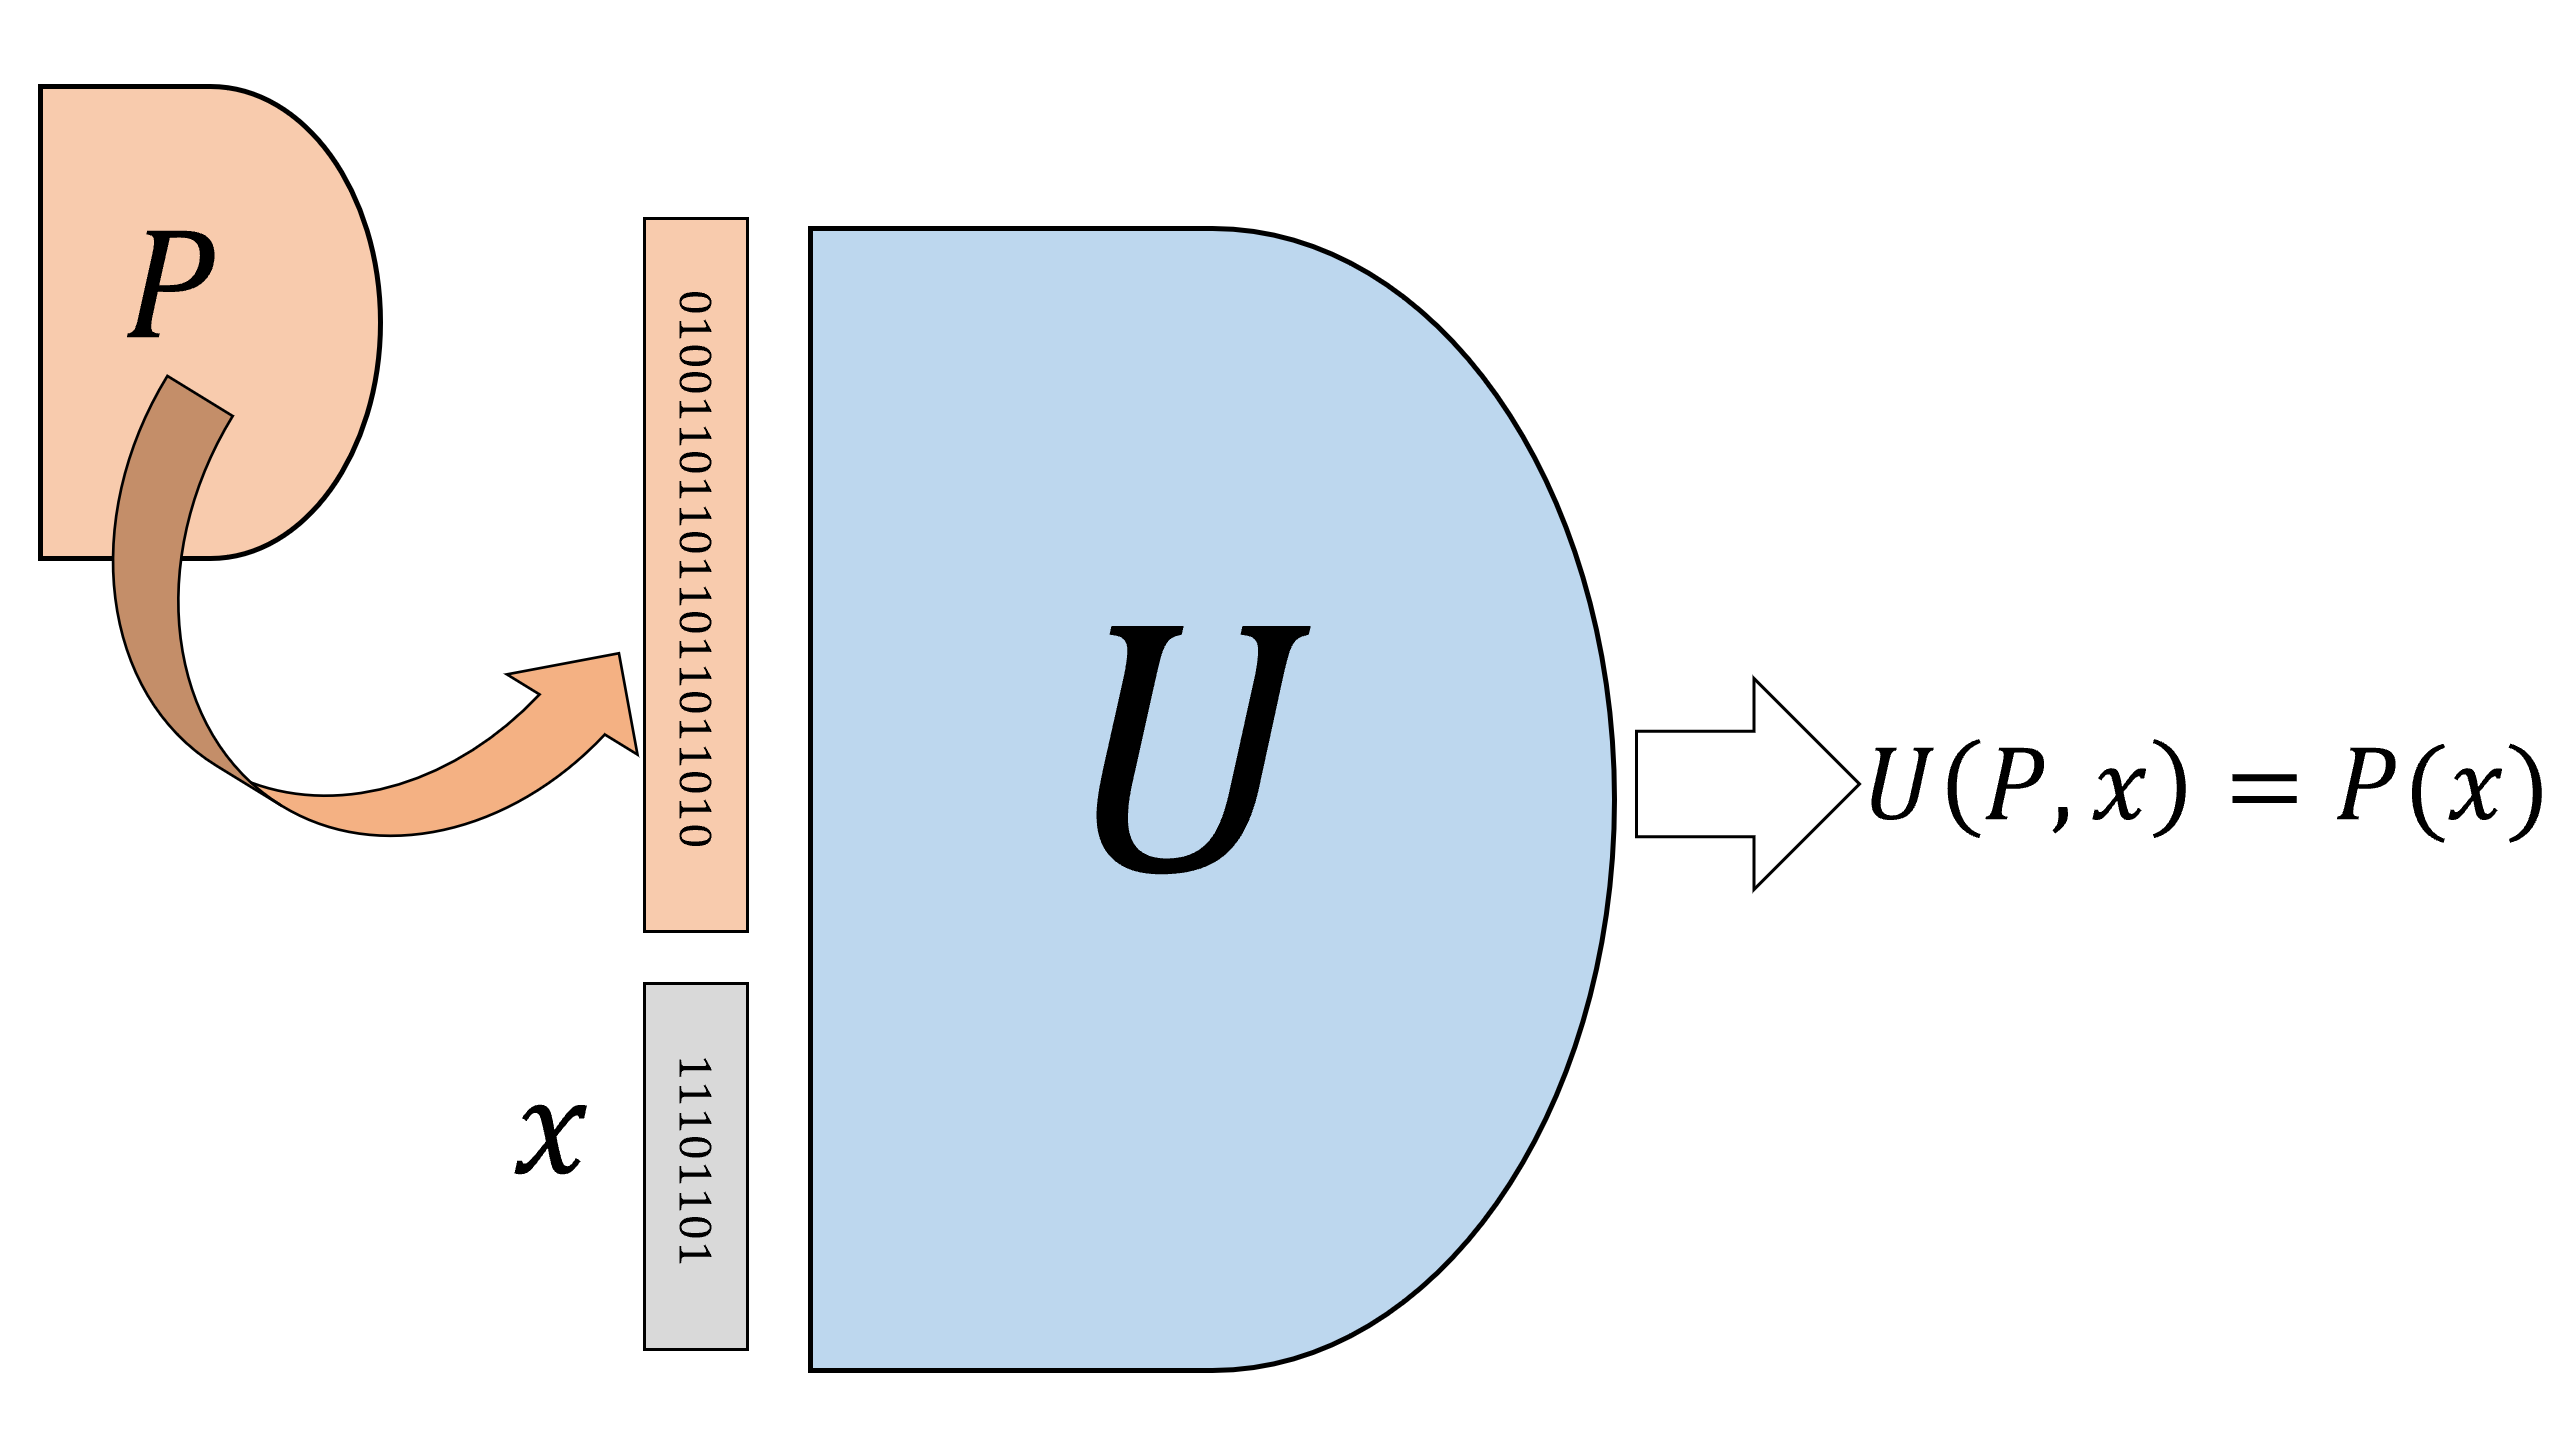
\includegraphics[width=\linewidth, height=1.5in, keepaspectratio]{../figure/universalcircuit.png}
\caption{A \emph{universal circuit} \(U\) is a circuit that gets as
input the description of an arbitrary (smaller) circuit \(P\) as a
binary string, and an input \(x\), and outputs the string \(P(x)\) which
is the evaluation of \(P\) on \(x\). We can also think of \(U\) as a
straight-line program that gets as input the code of a straight-line
program \(P\) and an input \(x\), and outputs \(P(x)\).}
\label{universalcircfig}
\end{marginfigure}

\subsection{Efficient universal
programs}\label{Efficient-universal-progr}

\cref{bounded-univ} establishes the existence of a NAND-CIRC program for
computing \(\ensuremath{\mathit{EVAL}}_{s,n,m}\), but it provides no
explicit bound on the size of this program. \cref{NAND-univ-thm}, which
we used to prove \cref{bounded-univ}, guarantees the existence of a
NAND-CIRC program whose size can be as large as \emph{exponential} in
the length of its input. This would mean that even for moderately small
values of \(s,n,m\) (for example \(n=100,s=300,m=1\)), computing
\(\ensuremath{\mathit{EVAL}}_{s,n,m}\) might require a NAND program with
more lines than there are atoms in the observable universe! Fortunately,
we can do much better than that. In fact, for every \(s,n,m\) there
exists a NAND-CIRC program for computing
\(\ensuremath{\mathit{EVAL}}_{s,n,m}\) with size that is
\emph{polynomial} in its input length. This is shown in the following
theorem.

\hypertarget{eff-bounded-univ}{}
\begin{theorem}[Efficient bounded universality of NAND-CIRC programs] \label[theorem]{eff-bounded-univ}

For every \(s,n,m \in \N\) there is a NAND-CIRC program of at most
\(O(s^2 \log s)\) lines that computes the function
\(\ensuremath{\mathit{EVAL}}_{s,n,m}:\{0,1\}^{S+n} \rightarrow \{0,1\}^m\)
defined above (where \(S\) is the number of bits needed to represent
programs of \(s\) lines).

\end{theorem}

\begin{pause} \label[pause]{If-you-havent-done-so-alr}

If you haven't done so already, now might be a good time to review \(O\)
notation in \cref{secbigohnotation}. In particular, an equivalent way to
state \cref{eff-bounded-univ} is that it says that there \emph{exists}
some number \(c>0\) such that \emph{for every} \(s,n,m \in \N\), there
exists a NAND-CIRC program \(P\) of at most \(c s^2 \log s\) lines that
computes the function \(\ensuremath{\mathit{EVAL}}_{s,n,m}\).

\end{pause}

Unlike \cref{bounded-univ}, \cref{eff-bounded-univ} is not a trivial
corollary of the fact that every finite function can be computed by some
circuit. Proving \cref{bounded-univ} requires us to present a concrete
NAND-CIRC program for computing the function
\(\ensuremath{\mathit{EVAL}}_{s,n,m}\). We will do so in several stages.

\begin{enumerate}
\def\labelenumi{\arabic{enumi}.}
\item
  First, we will describe the algorithm to evaluate
  \(\ensuremath{\mathit{EVAL}}_{s,n,m}\) in ``pseudo code''.
\item
  Then, we will show how we can write a program to compute
  \(\ensuremath{\mathit{EVAL}}_{s,n,m}\) in \emph{Python}. We will not
  use much about Python, and a reader that has familiarity with
  programming in any language should be able to follow along.
\item
  Finally, we will show how we can transform this Python program into a
  NAND-CIRC program.
\end{enumerate}

This approach yields much more than just proving
\cref{eff-bounded-univ}: we will see that it is in fact always possible
to transform (loop free) code in high level languages such as Python to
NAND-CIRC programs (and hence to Boolean circuits as well).

\subsection{A NAND-CIRC interpeter in
``pseudocode''}\label{A-NAND-CIRC-interpeter-in}

To prove \cref{eff-bounded-univ} it suffices to give a NAND-CIRC program
of \(O(s^2 \log s)\) lines that can evaluate NAND-CIRC programs of \(s\)
lines. Let us start by thinking how we would evaluate such programs if
we weren't restricted to only performing NAND operations. That is, let
us describe informally an \emph{algorithm} that on input \(n,m,s\), a
list of triples \(L\), and a string \(x\in \{0,1\}^n\), evaluates the
program represented by \((n,m,L)\) on the string \(x\).

\begin{pause} \label[pause]{It-would-be-highly-worthw}

It would be highly worthwhile for you to stop here and try to solve this
problem yourself. For example, you can try thinking how you would write
a program \texttt{NANDEVAL(n,m,s,L,x)} that computes this function in
the programming language of your choice.

\end{pause}

We will now describe such an algorithm. We assume that we have access to
a \emph{bit array} data structure that can store for every \(i\in [t]\)
a bit \(T_i \in \{0,1\}\). Specifically, if \texttt{Table} is a variable
holding this data structure, then we assume we can perform the
operations:

\begin{itemize}
\item
  \texttt{GET(Table,i)} which retrieves the bit corresponding to
  \texttt{i} in \texttt{Table}. The value of \texttt{i} is assumed to be
  an integer in \([t]\).
\item
  \texttt{Table = UPDATE(Table,i,b)} which updates \texttt{Table} so the
  the bit corresponding to \texttt{i} is now set to \texttt{b}. The
  value of \texttt{i} is assumed to be an integer in \([t]\) and
  \texttt{b} is a bit in \(\{0,1\}\).
\end{itemize}

\begin{algorithm}[Eval NAND-CIRC programs]
\label[algorithm]{evalnandcircalg} ~ \\ \noindent
\begin{algorithmic}[1]
\INPUT  Numbers $n,m,s$ and $t\leq 3s$, as well as  a list $L$ of $s$ triples of numbers in $[t]$, and  a string $x\in \{0,1\}^n$.
\OUTPUT  Evaluation of the program represented by $(n,m,L)$ on the \INPUT $x\in \{0,1\}^n$.
\STATE Let \texttt{Vartable} be table of size $t$
\FOR{$i$ in $[n]$}
\STATE \texttt{Vartable = UPDATE(Vartable,}$i$\texttt{,}$x_i$\texttt{)}
\ENDFOR
\FOR{$(i,j,k)$ in $L$}
\STATE $a \leftarrow$ \texttt{GET(Vartable,}$j$\texttt{)}
\STATE $b \leftarrow$ \texttt{GET(Vartable,}$k$\texttt{)}
\STATE \texttt{Vartable = UPDATE(Vartable,}$i$,\texttt{NAND(}$a$\texttt{,}$b$\texttt{))}
\ENDFOR
\FOR{$j$ in $[m]$}
\STATE $y_j \leftarrow$ \texttt{GET(Vartable,}$t-m+j$\texttt{)}
\ENDFOR
\RETURN $y_0,\ldots,y_{m-1}$
\end{algorithmic}
\end{algorithm}

\cref{evalnandcircalg} evaluates the program given to it as input one
line at a time, updating the \texttt{Vartable} table to contain the
value of each variable. At the end of the execution it outputs the
variables at positions \(t-m,t-m+1,\ldots,t-1\) which correspond to the
input variables.

\subsection{A NAND interpreter in Python}\label{nandevalpythonsec}

To make things more concrete, let us see how we implement
\cref{evalnandcircalg} in the \emph{Python} programming language. (There
is nothing special about Python. We could have easily presented a
corresponding function in JavaScript, C, OCaml, or any other programming
language.) We will construct a function \texttt{NANDEVAL} that on input
\(n,m,L,x\) will output the result of evaluating the program represented
by \((n,m,L)\) on \(x\). To keep things simple, we will not worry about
the case that \(L\) does not represent a valid program of \(n\) inputs
and \(m\) outputs. The code is presented in \cref{nandevalcode}.

\begin{figure*}

\classiccaptionstyle
\caption{Code for evaluating a NAND-CIRC program given in the list-of-tuples representation}
\label{nandevalcode}

\begin{framedcode}
def NANDEVAL(n,m,L,X):
    # Evaluate a NAND-CIRC program from list of tuple representation.
    s = len(L) # num of lines
    t = max(max(a,b,c) for (a,b,c) in L)+1 # max index in L + 1
    Vartable = [0] * t # initialize array

    # helper functions
    def GET(V,i): return V[i]
    def UPDATE(V,i,b):
        V[i]=b
        return V

    # load input values to Vartable:
    for i in range(n):
        Vartable = UPDATE(Vartable,i,X[i])

    # Run the program
    for (i,j,k) in L:
        a = GET(Vartable,j)
        b = GET(Vartable,k)
        c = NAND(a,b)
        Vartable = UPDATE(Vartable,i,c)

    # Return outputs Vartable[t-m], Vartable[t-m+1],....,Vartable[t-1]
    return [GET(Vartable,t-m+j) for j in range(m)]

# Test on XOR (2 inputs, 1 output)
L = ((2, 0, 1), (3, 0, 2), (4, 1, 2), (5, 3, 4))
print(NANDEVAL(2,1,L,(0,1))) # XOR(0,1)
# [1]
print(NANDEVAL(2,1,L,(1,1))) # XOR(1,1)
# [0]
\end{framedcode}
\end{figure*}

Accessing an element of the array \texttt{Vartable} at a given index
takes a constant number of basic operations. Hence (since \(n,m \leq s\)
and \(t \leq 3s\)), the program above will use \(O(s)\) basic
operations.\footnote{Python does not distinguish between lists and
  arrays, but allows constant time random access to an indexed elements
  to both of them. One could argue that if we allowed programs of truly
  unbounded length (e.g., larger than \(2^{64}\)) then the price would
  not be constant but logarithmic in the length of the array/lists, but
  the difference between \(O(s)\) and \(O(s \log s)\) will not be
  important for our discussions.}

\subsection{Constructing the NAND-CIRC interpreter in
NAND-CIRC}\label{Constructing-the-NAND-CIR}

We now turn to describing the proof of \cref{eff-bounded-univ}. To prove
the theorem it is not enough to give a Python program. Rather, we need
to show how we compute the function
\(\ensuremath{\mathit{EVAL}}_{s,n,m}\) using a \emph{NAND-CIRC program}.
In other words, our job is to transform, for every \(s,n,m\), the Python
code of \cref{nandevalpythonsec} to a NAND-CIRC program \(U_{s,n,m}\)
that computes the function \(\ensuremath{\mathit{EVAL}}_{s,n,m}\).

\begin{pause} \label[pause]{Before-reading-further-tr}

Before reading further, try to think how \emph{you} could give a
``constructive proof'' of \cref{eff-bounded-univ}. That is, think of how
you would write, in the programming language of your choice, a function
\texttt{universal(s,n,m)} that on input \(s,n,m\) outputs the code for
the NAND-CIRC program \(U_{s,n,m}\) such that \(U_{s,n,m}\) computes
\(\ensuremath{\mathit{EVAL}}_{s,n,m}\). There is a subtle but crucial
difference between this function and the Python \texttt{NANDEVAL}
program described above. Rather than actually evaluating a given program
\(P\) on some input \(w\), the function \texttt{universal} should output
the \emph{code} of a NAND-CIRC program that computes the map
\((P,x) \mapsto P(x)\).

\end{pause}

Our construction will follow very closely the Python implementation of
\texttt{EVAL} above. We will use variables
\texttt{Vartable[}\(0\)\texttt{]},\(\ldots\),\texttt{Vartable[}\(2^\ell-1\)\texttt{]},
where \(\ell = \ceil{\log 3s}\) to store our variables. However, NAND
doesn't have integer-valued variables, so we cannot write code such as
\texttt{Vartable[i]} for some variable \texttt{i}. However, we
\emph{can} implement the function \texttt{GET(Vartable,i)} that outputs
the \texttt{i}-th bit of the array \texttt{Vartable}. Indeed, this is
nothing but the function \(\ensuremath{\mathit{LOOKUP}}_\ell\) that we
have seen in \cref{lookup-thm}!

\begin{pause} \label[pause]{Please-make-sure-that-you}

Please make sure that you understand why \texttt{GET} and
\(\ensuremath{\mathit{LOOKUP}}_\ell\) are the same function.

\end{pause}

We saw that we can compute \(\ensuremath{\mathit{LOOKUP}}_\ell\) in time
\(O(2^\ell) = O(s)\) for our choice of \(\ell\).

For every \(\ell\), let
\(\ensuremath{\mathit{UPDATE}}_\ell:\{0,1\}^{2^\ell + \ell +1} \rightarrow \{0,1\}^{2^\ell}\)
correspond to the \texttt{UPDATE} function for arrays of length
\(2^\ell\). That is, on input \(V\in \{0,1\}^{2^\ell}\) ,
\(i\in \{0,1\}^\ell\), \(b\in \{0,1\}\),
\(\ensuremath{\mathit{UPDATE}}_\ell(V,b,i)\) is equal to
\(V' \in \{0,1\}^{2^\ell}\) such that \[
V'_j = \begin{cases} V_j & j \neq i \\ b & j = 1 \end{cases}
\] where we identify the string \(i \in \{0,1\}^\ell\) with a number in
\(\{0,\ldots, 2^{\ell}-1 \}\) using the binary representation. We can
compute \(\ensuremath{\mathit{UPDATE}}_\ell\) using an
\(O(2^\ell \ell)=(s \log s)\) line NAND-CIRC program as as follows:

\begin{enumerate}
\def\labelenumi{\arabic{enumi}.}
\item
  For every \(j\in [2^\ell]\), there is an \(O(\ell)\) line NAND-CIRC
  program to compute the function
  \(\ensuremath{\mathit{EQUALS}}_j: \{0,1\}^\ell \rightarrow \{0,1\}\)
  that on input \(i\) outputs \(1\) if and only if \(i\) is equal to
  (the binary representation of) \(j\). (We leave verifying this as
  \cref{equals} and \cref{equalstwo}.)
\item
  We have seen that we can compute the function
  \(\ensuremath{\mathit{IF}}:\{0,1\}^3 \rightarrow \{0,1\}\) such that
  \(\ensuremath{\mathit{IF}}(a,b,c)\) equals \(b\) if \(a=1\) and \(c\)
  if \(a=0\).
\end{enumerate}

Together, this means that we can compute \texttt{UPDATE} (using some
``syntactic sugar'' for bounded length loops) as follows:

\begin{code}
def UPDATE_ell(V,i,b):
    # Get V[0]...V[2^ell-1], i in {0,1}^ell, b in {0,1}
    # Return NewV[0],...,NewV[2^ell-1]
    # updated array with NewV[i]=b and all
    # else same as V
    for j in range(2**ell): # j = 0,1,2,....,2^ell -1
        a = EQUALS_j(i)
        NewV[j] = IF(a,b,V[j])
    return NewV
\end{code}

Since the loop over \texttt{j} in \texttt{UPDATE} is run \(2^\ell\)
times, and computing \texttt{EQUALS\_j} takes \(O(\ell)\) lines, the
total number of lines to compute \texttt{UPDATE} is
\(O(2^\ell \cdot \ell) = O(s \log s)\). Once we can compute \texttt{GET}
and \texttt{UPDATE}, the rest of the implementation amounts to ``book
keeping'' that needs to be done carefully, but is not too insightful,
and hence we omit the full details. Since we run \texttt{GET} and
\texttt{UPDATE} \(s\) times, the total number of lines for computing
\(\ensuremath{\mathit{EVAL}}_{s,n,m}\) is
\(O(s^2) + O(s^2 \log s) = O(s^2 \log s)\). This completes (up to the
omitted details) the proof of \cref{eff-bounded-univ}.

\hypertarget{quasilinearevalrem}{}
\begin{remark}[Improving to quasilinear overhead (advanced optional note)] \label[remark]{quasilinearevalrem}

The NAND-CIRC program above is less efficient than its Python
counterpart, since NAND does not offer arrays with efficient random
access. Hence for example the \texttt{LOOKUP} operation on an array of
\(s\) bits takes \(\Omega(s)\) lines in NAND even though it takes
\(O(1)\) steps (or maybe \(O(\log s)\) steps, depending on how we count)
in \emph{Python}.

It turns out that it is possible to improve the bound of
\cref{eff-bounded-univ}, and evaluate \(s\) line NAND-CIRC programs
using a NAND-CIRC program of \(O(s \log s)\) lines. The key is to
consider the description of NAND-CIRC programs as circuits, and in
particular as directed acyclic graphs (DAGs) of bounded in-degree. A
universal NAND-CIRC program \(U_s\) for \(s\) line programs will
correspond to a \emph{universal graph} \(H_s\) for such \(s\) vertex
DAGs. We can think of such a graph \(U_s\) as fixed ``wiring'' for a
communication network, that should be able to accommodate any arbitrary
pattern of communication between \(s\) vertices (where this pattern
corresponds to an \(s\) line NAND-CIRC program). It turns out that such
efficient \href{https://goo.gl/NnkkjM}{routing networks} exist that
allow embedding any \(s\) vertex circuit inside a universal graph of
size \(O(s \log s)\), see the bibliographical notes
\cref{bibnotescodeasdata} for more on this issue.

\end{remark}

\section{A Python interpreter in NAND-CIRC
(discussion)}\label{A-Python-interpreter-in-N}

To prove \cref{eff-bounded-univ} we essentially translated every line of
the Python program for \texttt{EVAL} into an equivalent NAND-CIRC
snippet. However none of our reasoning was specific to the particular
function \(\ensuremath{\mathit{EVAL}}\). It is possible to translate
\emph{every} Python program into an equivalent NAND-CIRC program of
comparable efficiency. (More concretely, if the Python program takes
\(T(n)\) operations on inputs of length at most \(n\) then there exists
NAND-CIRC program of \(O(T(n) \log T(n))\) lines that agrees with the
Python program on inputs of length \(n\).) Actually doing so requires
taking care of many details and is beyond the scope of this book, but
let me try to convince you why you should believe it is possible in
principle.

For starters, one can use
\href{https://en.wikipedia.org/wiki/CPython}{CPython} (the reference
implementation for Python), to evaluate every Python program using a
\texttt{C} program. We can combine this with a C compiler to transform a
Python program to various flavors of ``machine language''. So, to
transform a Python program into an equivalent NAND-CIRC program, it is
enough to show how to transform a \emph{machine language} program into
an equivalent NAND-CIRC program. One minimalistic (and hence convenient)
family of machine languages is known as the \emph{ARM architecture}
which powers many mobile devices including essentially all Android
devices.\footnote{ARM stands for ``Advanced RISC Machine'' where RISC in
  turn stands for ``Reduced instruction set computer''.} There are even
simpler machine languages, such as the
\href{https://github.com/frasercrmck/llvm-leg}{LEG architecture} for
which a backend for the \href{http://llvm.org/}{LLVM compiler} was
implemented (and hence can be the target of compiling any of
\href{https://en.wikipedia.org/wiki/LLVM\#Front_ends}{large and growing
list} of languages that this compiler supports). Other examples include
the \href{http://www.scipr-lab.org/doc/TinyRAM-spec-0.991.pdf}{TinyRAM}
architecture (motivated by interactive proof systems that we will
discuss in \cref{chapproofs}) and the teaching-oriented
\href{https://www.ece.umd.edu/~blj/RiSC/}{Ridiculously Simple Computer}
architecture. Going one by one over the instruction sets of such
computers and translating them to NAND snippets is no fun, but it is a
feasible thing to do. In fact, ultimately this is very similar to the
transformation that takes place in converting our high level code to
actual silicon gates that are not so different from the operations of a
NAND-CIRC program. Indeed, tools such as
\href{http://www.myhdl.org/}{MyHDL} that transform ``Python to Silicon''
can be used to convert a Python program to a NAND-CIRC program.

The NAND-CIRC programming language is just a teaching tool, and by no
means do I suggest that writing NAND-CIRC programs, or compilers to
NAND-CIRC, is a practical, useful, or enjoyable activity. What I do want
is to make sure you understand why it \emph{can} be done, and to have
the confidence that if your life (or at least your grade) depended on
it, then you would be able to do this. Understanding how programs in
high level languages such as Python are eventually transformed into
concrete low-level representation such as NAND is fundamental to
computer science.

The astute reader might notice that the above paragraphs only outlined
why it should be possible to find for every \emph{particular}
Python-computable function \(f\), a \emph{particular} comparably
efficient NAND-CIRC program \(P\) that computes \(f\). But this still
seems to fall short of our goal of writing a ``Python interpreter in
NAND'' which would mean that for every parameter \(n\), we come up with
a \emph{single} NAND-CIRC program \(\ensuremath{\mathit{UNIV}}_s\) such
that given a description of a Python program \(P\), a particular input
\(x\), and a bound \(T\) on the number of operations (where the lengths
of \(P\) and \(x\) and the value of \(T\) are all at most \(s\)) returns
the result of executing \(P\) on \(x\) for at most \(T\) steps. After
all, the transformation above takes every Python program into a
\emph{different} NAND-CIRC program, and so does not yield ``one
NAND-CIRC program to rule them all'' that can evaluate every Python
program up to some given complexity. However, we can in fact obtain one
NAND-CIRC program to evaluate \emph{arbitrary} Python programs. The
reason is that there exists a Python interpreter \emph{in Python}: a
Python program \(U\) that takes a bit string, interprets it as Python
code, and then runs that code. Hence, we only need to show a NAND-CIRC
program \(U^*\) that computes the same function as the particular Python
program \(U\), and this will give us a way to evaluate \emph{all} Python
programs.

What we are seeing time and again is the notion of \emph{universality}
or \emph{self reference} of computation, which is the sense that all
reasonably rich models of computation are expressive enough that they
can ``simulate themselves''. The importance of this phenomenon to both
the theory and practice of computing, as well as far beyond it,
including the foundations of mathematics and basic questions in science,
cannot be overstated.

\section{The physical extended Church-Turing thesis
(discussion)}\label{PECTTsec}

We've seen that NAND gates (and other Boolean operations) can be
implemented using very different systems in the physical world. What
about the reverse direction? Can NAND-CIRC programs simulate any
physical computer?

We can take a leap of faith and stipulate that Boolean circuits (or
equivalently NAND-CIRC programs) do actually encapsulate \emph{every}
computation that we can think of. Such a statement (in the realm of
infinite functions, which we'll encounter in \cref{chaploops}) is
typically attributed to Alonzo Church and Alan Turing, and in that
context is known as the \emph{Church Turing Thesis}. As we will discuss
in future lectures, the Church-Turing Thesis is not a mathematical
theorem or conjecture. Rather, like theories in physics, the
Church-Turing Thesis is about mathematically modeling the real world. In
the context of finite functions, we can make the following informal
hypothesis or prediction:

\begin{quote}
\textbf{``Physical Extended Church-Turing Thesis'' (PECTT):} \emph{If a
function \(F:\{0,1\}^n \rightarrow \{0,1\}^m\) can be computed in the
physical world using \(s\) amount of ``physical resources'' then it can
be computed by a Boolean circuit program of roughly \(s\) gates.}
\end{quote}

A priori it might seem rather extreme to hypothesize that our meager
model of NAND-CIRC programs or Boolean circuits captures all possible
physical computation. But yet, in more than a century of computing
technologies, no one has yet built any scalable computing device that
challenges this hypothesis.

We now discuss the ``fine print'' of the PECTT in more detail, as well
as the (so far unsuccessful) challenges that have been raised against
it. There is no single universally-agreed-upon formalization of
``roughly \(s\) physical resources'', but we can approximate this notion
by considering the size of any physical computing device and the time it
takes to compute the output, and ask that any such device can be
simulated by a Boolean circuit with a number of gates that is a
polynomial (with not too large exponent) in the size of the system and
the time it takes it to operate.

In other words, we can phrase the PECTT as stipulating that any function
that can be computed by a device that takes a certain volume \(V\) of
space and requires \(t\) time to complete the computation, must be
computable by a Boolean circuit with a number of gates \(p(V,t)\) that
is polynomial in \(V\) and \(t\).

The exact form of the function \(p(V,t)\) is not universally agreed upon
but it is generally accepted that if \(f:\{0,1\}^n \rightarrow \{0,1\}\)
is an \emph{exponentially hard} function, in the sense that it has no
NAND-CIRC program of fewer than, say, \(2^{n/2}\) lines, then a
demonstration of a physical device that can compute in the real world
\(f\) for moderate input lengths (e.g., \(n=500\)) would be a violation
of the PECTT.

\hypertarget{concretepectt}{}
\begin{remark}[Advanced note: making PECTT concrete (advanced, optional)] \label[remark]{concretepectt}

We can attempt a more exact phrasing of the PECTT as follows. Suppose
that \(Z\) is a physical system that accepts \(n\) binary stimuli and
has a binary output, and can be enclosed in a sphere of volume \(V\). We
say that the system \(Z\) \emph{computes} a function
\(f:\{0,1\}^n \rightarrow \{0,1\}\) within \(t\) seconds if whenever we
set the stimuli to some value \(x\in \{0,1\}^n\), if we measure the
output after \(t\) seconds then we obtain \(f(x)\).

One can then phrase the PECTT as stipulating that if there exists such a
system \(Z\) that computes \(F\) within \(t\) seconds, then there exists
a NAND-CIRC program that computes \(F\) and has at most \(\alpha(Vt)^2\)
lines, where \(\alpha\) is some normalization constant. (We can also
consider variants where we use \href{https://goo.gl/ALgbVS}{surface
area} instead of volume, or take \((Vt)\) to a different power than
\(2\). However, none of these choices makes a qualitative difference to
the discussion below.) In particular, suppose that
\(f:\{0,1\}^n \rightarrow \{0,1\}\) is a function that requires
\(2^n/(100n)>2^{0.8n}\) lines for any NAND-CIRC program (such a function
exists by \cref{counting-lb}). Then the PECTT would imply that either
the volume or the time of a system that computes \(F\) will have to be
at least \(2^{0.2 n}/\sqrt{\alpha}\). Since this quantity grows
\emph{exponentially} in \(n\), it is not hard to set parameters so that
even for moderately large values of \(n\), such a system could not fit
in our universe.

To fully make the PECTT concrete, we need to decide on the units for
measuring time and volume, and the normalization constant \(\alpha\).
One conservative choice is to assume that we could squeeze computation
to the absolute physical limits (which are many orders of magnitude
beyond current technology). This corresponds to setting \(\alpha=1\) and
using the \href{https://goo.gl/gkpmBF}{Planck units} for volume and
time. The \emph{Planck length} \(\ell_P\) (which is, roughly speaking,
the shortest distance that can theoretically be measured) is roughly
\(2^{-120}\) meters. The \emph{Planck time} \(t_P\) (which is the time
it takes for light to travel one Planck length) is about \(2^{-150}\)
seconds. In the above setting, if a function \(F\) takes, say, 1KB of
input (e.g., roughly \(10^4\) bits, which can encode a \(100\) by
\(100\) bitmap image), and requires at least
\(2^{0.8 n}= 2^{0.8 \cdot 10^4}\) NAND lines to compute, then any
physical system that computes it would require either volume of
\(2^{0.2\cdot 10^4}\) Planck length cubed, which is more than
\(2^{1500}\) meters cubed or take at least \(2^{0.2 \cdot 10^4}\) Planck
Time units, which is larger than \(2^{1500}\) seconds. To get a sense of
how big that number is, note that the universe is only about \(2^{60}\)
seconds old, and its observable radius is only roughly \(2^{90}\)
meters. The above discussion suggests that it is possible to
\emph{empirically falsify} the PECTT by presenting a
smaller-than-universe-size system that computes such a function.

There are of course several hurdles to refuting the PECTT in this way,
one of which is that we can't actually test the system on all possible
inputs. However, it turns out that we can get around this issue using
notions such as \emph{interactive proofs} and \emph{program checking}
that we might encounter later in this book. Another, perhaps more
salient problem, is that while we know many hard functions exist, at the
moment there is \emph{no single explicit function}
\(F:\{0,1\}^n \rightarrow \{0,1\}\) for which we can \emph{prove} an
\(\omega(n)\) (let alone \(\Omega(2^n/n)\)) lower bound on the number of
lines that a NAND-CIRC program needs to compute it.

\end{remark}

\subsection{Attempts at refuting the
PECTT}\label{Attempts-at-refuting-the-}

One of the admirable traits of mankind is the refusal to accept
limitations. In the best case this is manifested by people achieving
longstanding ``impossible'' challenges such as heavier-than-air flight,
putting a person on the moon, circumnavigating the globe, or even
resolving
\href{https://en.wikipedia.org/wiki/Fermat\%27s_Last_Theorem}{Fermat's
Last Theorem}. In the worst case it is manifested by people continually
following the footsteps of previous failures to try to do
proven-impossible tasks such as build a
\href{https://en.wikipedia.org/wiki/Perpetual_motion}{perpetual motion
machine}, \href{https://en.wikipedia.org/wiki/Angle_trisection}{trisect
an angle} with a compass and straightedge, or refute
\href{https://en.wikipedia.org/wiki/Bell\%27s_theorem}{Bell's
inequality}. The Physical Extended Church Turing thesis (in its various
forms) has attracted both types of people. Here are some physical
devices that have been speculated to achieve computational tasks that
cannot be done by not-too-large NAND-CIRC programs:

\begin{itemize}
\item
  \textbf{Spaghetti sort:} One of the first lower bounds that Computer
  Science students encounter is that sorting \(n\) numbers requires
  making \(\Omega(n \log n)\) comparisons. The ``spaghetti sort'' is a
  description of a proposed ``mechanical computer'' that would do this
  faster. The idea is that to sort \(n\) numbers \(x_1,\ldots,x_n\), we
  could cut \(n\) spaghetti noodles into lengths \(x_1,\ldots,x_n\), and
  then if we simply hold them together in our hand and bring them down
  to a flat surface, they will emerge in sorted order. There are a great
  many reasons why this is not truly a challenge to the PECTT
  hypothesis, and I will not ruin the reader's fun in finding them out
  by her or himself.
\item
  \textbf{Soap bubbles:} One function
  \(F:\{0,1\}^n \rightarrow \{0,1\}\) that is conjectured to require a
  large number of NAND lines to solve is the \emph{Euclidean Steiner
  Tree} problem. This is the problem where one is given \(m\) points in
  the plane \((x_1,y_1),\ldots,(x_m,y_m)\) (say with integer coordinates
  ranging from \(1\) till \(m\), and hence the list can be represented
  as a string of \(n=O(m \log m)\) size) and some number \(K\). The goal
  is to figure out whether it is possible to connect all the points by
  line segments of total length at most \(K\). This function is
  conjectured to be hard because it is \emph{NP complete} - a concept
  that we'll encounter later in this course - and it is in fact
  reasonable to conjecture that as \(m\) grows, the number of NAND lines
  required to compute this function grows \emph{exponentially} in \(m\),
  meaning that the PECTT would predict that if \(m\) is sufficiently
  large (such as few hundreds or so) then no physical device could
  compute \(F\). Yet, some people claimed that there is in fact a very
  simple physical device that could solve this problem, that can be
  constructed using some wooden pegs and soap. The idea is that if we
  take two glass plates, and put \(m\) wooden pegs between them in the
  locations \((x_1,y_1),\ldots,(x_m,y_m)\) then bubbles will form whose
  edges touch those pegs in a way that will minimize the total energy
  which turns out to be a function of the total length of the line
  segments. The problem with this device is that nature, just like
  people, often gets stuck in ``local optima''. That is, the resulting
  configuration will not be one that achieves the absolute minimum of
  the total energy but rather one that can't be improved with local
  changes.
  \href{http://www.scottaaronson.com/papers/npcomplete.pdf}{Aaronson}
  has carried out actual experiments (see \cref{aaronsonsoapfig}), and
  saw that while this device often is successful for three or four pegs,
  it starts yielding suboptimal results once the number of pegs grows
  beyond that.
\end{itemize}


\begin{marginfigure}
\centering
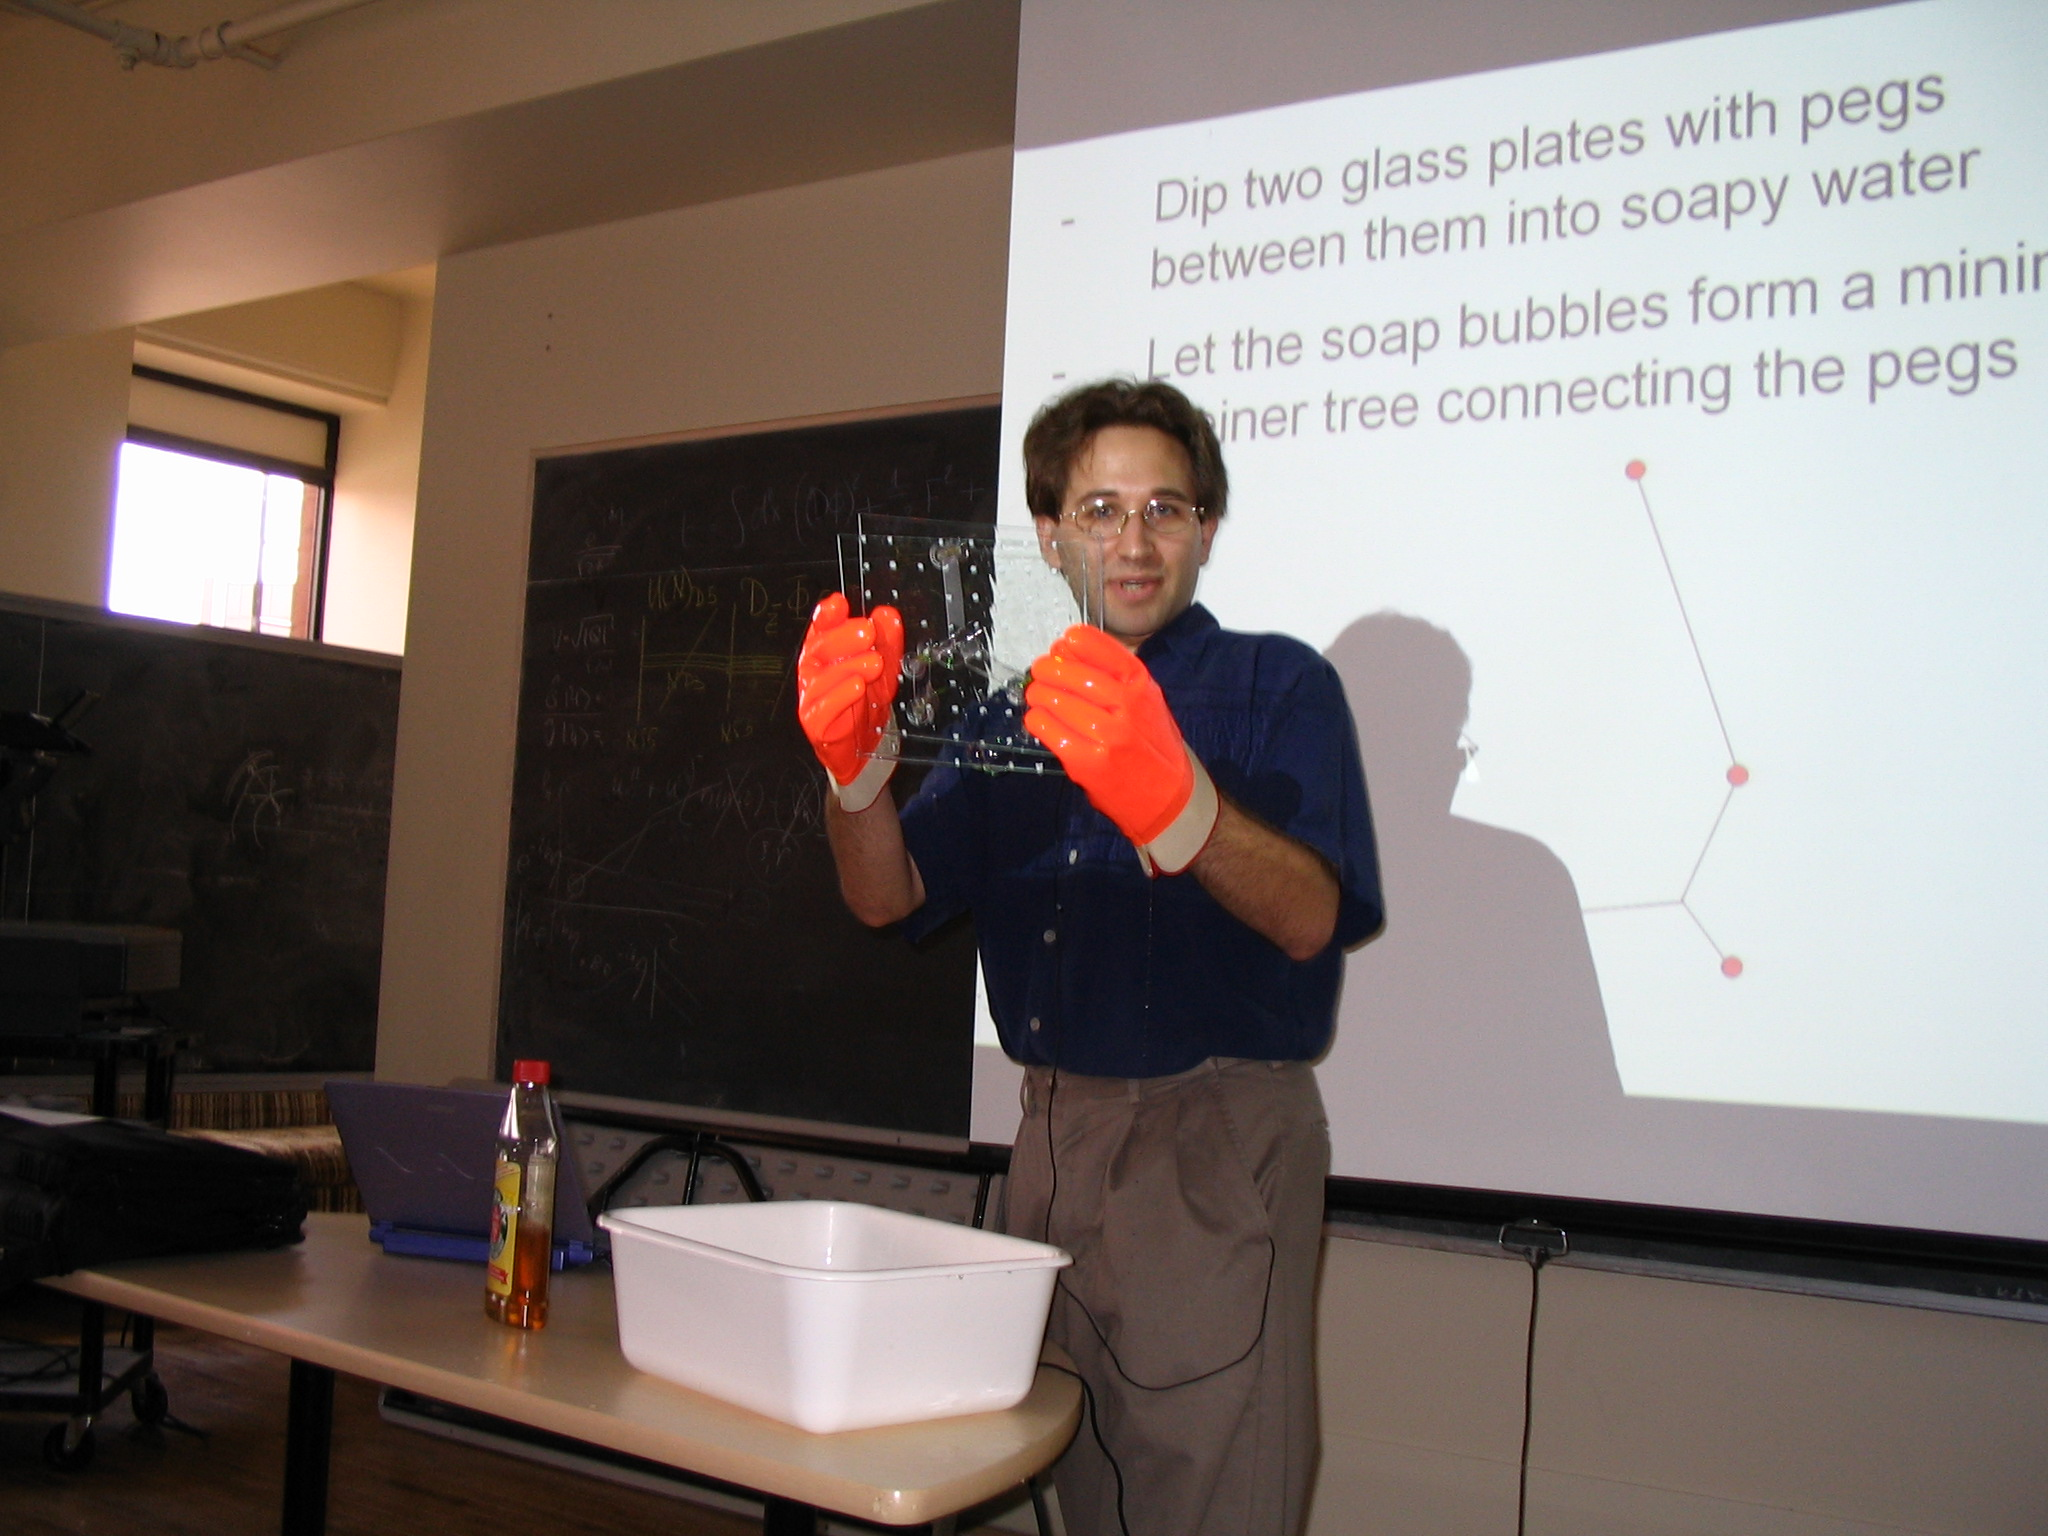
\includegraphics[width=\linewidth, height=1.5in, keepaspectratio]{../figure/aaronsonsoapbubble.jpg}
\caption{Scott Aaronson
\href{http://www.scottaaronson.com/blog/?p=266}{tests} a candidate
device for computing Steiner trees using soap bubbles.}
\label{aaronsonsoapfig}
\end{marginfigure}

\begin{itemize}
\item
  \textbf{DNA computing.} People have suggested using the properties of
  DNA to do hard computational problems. The main advantage of DNA is
  the ability to potentially encode a lot of information in a relatively
  small physical space, as well as compute on this information in a
  highly parallel manner. At the time of this writing, it was
  \href{http://science.sciencemag.org/content/337/6102/1628.full}{demonstrated}
  that one can use DNA to store about \(10^{16}\) bits of information in
  a region of radius about a millimeter, as opposed to about \(10^{10}\)
  bits with the best known hard disk technology. This does not posit a
  real challenge to the PECTT but does suggest that one should be
  conservative about the choice of constant and not assume that current
  hard disk + silicon technologies are the absolute best
  possible.\footnote{We were extremely conservative in the suggested
    parameters for the PECTT, having assumed that as many as
    \(\ell_P^{-2}10^{-6} \sim 10^{61}\) bits could potentially be stored
    in a millimeter radius region.}
\item
  \textbf{Continuous/real computers.} The physical world is often
  described using continuous quantities such as time and space, and
  people have suggested that analog devices might have direct access to
  computing with real-valued quantities and would be inherently more
  powerful than discrete models such as NAND machines. Whether the
  ``true'' physical world is continuous or discrete is an open question.
  In fact, we do not even know how to precisely \emph{phrase} this
  question, let alone answer it. Yet, regardless of the answer, it seems
  clear that the effort to measure a continuous quantity grows with the
  level of accuracy desired, and so there is no ``free lunch'' or way to
  bypass the PECTT using such machines (see also
  \href{http://www.cs.princeton.edu/~ken/MCS86.pdf}{this paper}).
  Related to that are proposals known as ``hypercomputing'' or ``Zeno's
  computers'' which attempt to use the continuity of time by doing the
  first operation in one second, the second one in half a second, the
  third operation in a quarter second and so on.. These fail for a
  similar reason to the one guaranteeing that Achilles will eventually
  catch the tortoise despite the original Zeno's paradox.
\item
  \textbf{Relativity computer and time travel.} The formulation above
  assumed the notion of time, but under the theory of relativity time is
  in the eye of the observer. One approach to solve hard problems is to
  leave the computer to run for a lot of time from \emph{his}
  perspective, but to ensure that this is actually a short while from
  \emph{our} perspective. One approach to do so is for the user to start
  the computer and then go for a quick jog at close to the speed of
  light before checking on its status. Depending on how fast one goes,
  few seconds from the point of view of the user might correspond to
  centuries in computer time (it might even finish updating its Windows
  operating system!). Of course the catch here is that the energy
  required from the user is proportional to how close one needs to get
  to the speed of light. A more interesting proposal is to use time
  travel via \emph{closed timelike curves (CTCs)}. In this case we could
  run an arbitrarily long computation by doing some calculations,
  remembering the current state, and then travelling back in time to
  continue where we left off. Indeed, if CTCs exist then we'd probably
  have to revise the PECTT (though in this case I will simply travel
  back in time and edit these notes, so I can claim I never conjectured
  it in the first place\ldots)
\item
  \textbf{Humans.} Another computing system that has been proposed as a
  counterexample to the PECTT is a 3 pound computer of about 0.1m
  radius, namely the human brain. Humans can walk around, talk, feel,
  and do other things that are not commonly done by NAND-CIRC programs,
  but can they compute partial functions that NAND-CIRC programs cannot?
  There are certainly computational tasks that \emph{at the moment}
  humans do better than computers (e.g., play some
  \href{http://www.theverge.com/2016/11/4/13518210/deepmind-starcraft-ai-google-blizzard}{video
  games}, at the moment), but based on our current understanding of the
  brain, humans (or other animals) have no \emph{inherent} computational
  advantage over computers. The brain has about \(10^{11}\) neurons,
  each operating at a speed of about \(1000\) operations per seconds.
  Hence a rough first approximation is that a Boolean circuit of about
  \(10^{14}\) gates could simulate one second of a brain's
  activity.\footnote{This is a very rough approximation that could be
    wrong to a few orders of magnitude in either direction. For one,
    there are other structures in the brain apart from neurons that one
    might need to simulate, hence requiring higher overhead. On the
    other hand, it is by no mean clear that we need to fully clone the
    brain in order to achieve the same computational tasks that it does.}
  Note that the fact that such a circuit (likely) exists does not mean
  it is easy to \emph{find} it. After all, constructing this circuit
  took evolution billions of years. Much of the recent efforts in
  artificial intelligence research is focused on finding programs that
  replicate some of the brain's capabilities and they take massive
  computational effort to discover, these programs often turn out to be
  much smaller than the pessimistic estimates above. For example, at the
  time of this writing, Google's
  \href{https://arxiv.org/pdf/1609.08144.pdf}{neural network for machine
  translation} has about \(10^4\) nodes (and can be simulated by a
  NAND-CIRC program of comparable size). Philosophers, priests and many
  others have since time immemorial argued that there is something about
  humans that cannot be captured by mechanical devices such as
  computers; whether or not that is the case, the evidence is thin that
  humans can perform computational tasks that are inherently impossible
  to achieve by computers of similar complexity.\footnote{There are some
    well known scientists that have
    \href{http://www.telegraph.co.uk/science/2017/03/14/can-solve-chess-problem-holds-key-human-consciousness/}{advocated}
    that humans have inherent computational advantages over computers.
    See also \href{https://arxiv.org/abs/1508.05929}{this}.}
\item
  \textbf{Quantum computation.} The most compelling attack on the
  Physical Extended Church Turing Thesis comes from the notion of
  \emph{quantum computing}. The idea was initiated by the observation
  that systems with strong quantum effects are very hard to simulate on
  a computer. Turning this observation on its head, people have proposed
  using such systems to perform computations that we do not know how to
  do otherwise. At the time of this writing, Scalable quantum computers
  have not yet been built, but it is a fascinating possibility, and one
  that does not seem to contradict any known law of nature. We will
  discuss quantum computing in much more detail in \cref{quantumchap}.
  Modeling quantum computation involves extending the model of Boolean
  circuits into \emph{Quantum circuits} that have one more (very
  special) gate. However, the main takeaway is that while quantum
  computing does suggest we need to amend the PECTT, it does \emph{not}
  require a complete revision of our worldview. Indeed, almost all of
  the content of this book remains the same regardless of whether the
  underlying computational model is Boolean circuits or quantum
  circuits.
\end{itemize}

\hypertarget{pcettcrypto}{}
\begin{remark}[Physical Extended Church-Turing Thesis and Cryptography] \label[remark]{pcettcrypto}

While even the precise phrasing of the PECTT, let alone understanding
its correctness, is still a subject of active research, some variants of
it are already implicitly assumed in practice. Governments, companies,
and individuals currently rely on \emph{cryptography} to protect some of
their most precious assets, including state secrets, control of weapon
systems and critical infrastructure, securing commerce, and protecting
the confidentiality of personal information. In applied cryptography,
one often encounters statements such as ``cryptosystem \(X\) provides
128 bits of security''. What such a statement really means is that
\textbf{(a)} it is conjectured that there is no Boolean circuit (or,
equivalently, a NAND-CIRC program) of size much smaller than \(2^{128}\)
that can break \(X\), and \textbf{(b)} we assume that no other physical
mechanism can do better, and hence it would take roughly a \(2^{128}\)
amount of ``resources'' to break \(X\). We say ``conjectured'' and not
``proved'' because, while we can phrase the statement that breaking the
system cannot be done by an \(s\)-gate circuit as a precise mathematical
conjecture, at the moment we are unable to \emph{prove} such a statement
for any non-trivial cryptosystem. This is related to the \(\mathbf{P}\)
vs \(\mathbf{NP}\) question we will discuss in future chapters. We will
explore Cryptography in \cref{chapcryptography}.

\end{remark}

\begin{recap} \label[recap]{We-can-think-of-programs-}

\begin{itemize}
\tightlist
\item
  We can think of programs both as describing a \emph{process}, as well
  as simply a list of symbols that can be considered as \emph{data} that
  can be fed as input to other programs.
\item
  We can write a NAND-CIRC program that evaluates arbitrary NAND-CIRC
  programs (or equivalently a circuit that evaluates other circuits).
  Moreover, the efficiency loss in doing so is not too large.
\item
  We can even write a NAND-CIRC program that evaluates programs in other
  programming languages such as Python, C, Lisp, Java, Go, etc.
\item
  By a leap of faith, we could hypothesize that the number of gates in
  the smallest circuit that computes a function \(f\) captures roughly
  the amount of physical resources required to compute \(f\). This
  statement is known as the \emph{Physical Extended Church-Turing Thesis
  (PECTT)}.
\item
  Boolean circuits (or equivalently AON-CIRC or NAND-CIRC programs)
  capture a surprisingly wide array of computational models. The
  strongest currently known challenge to the PECTT comes from the
  potential for using quantum mechanical effects to speed-up
  computation, a model known as \emph{quantum computers}.
\end{itemize}

\end{recap}


\begin{figure}
\centering
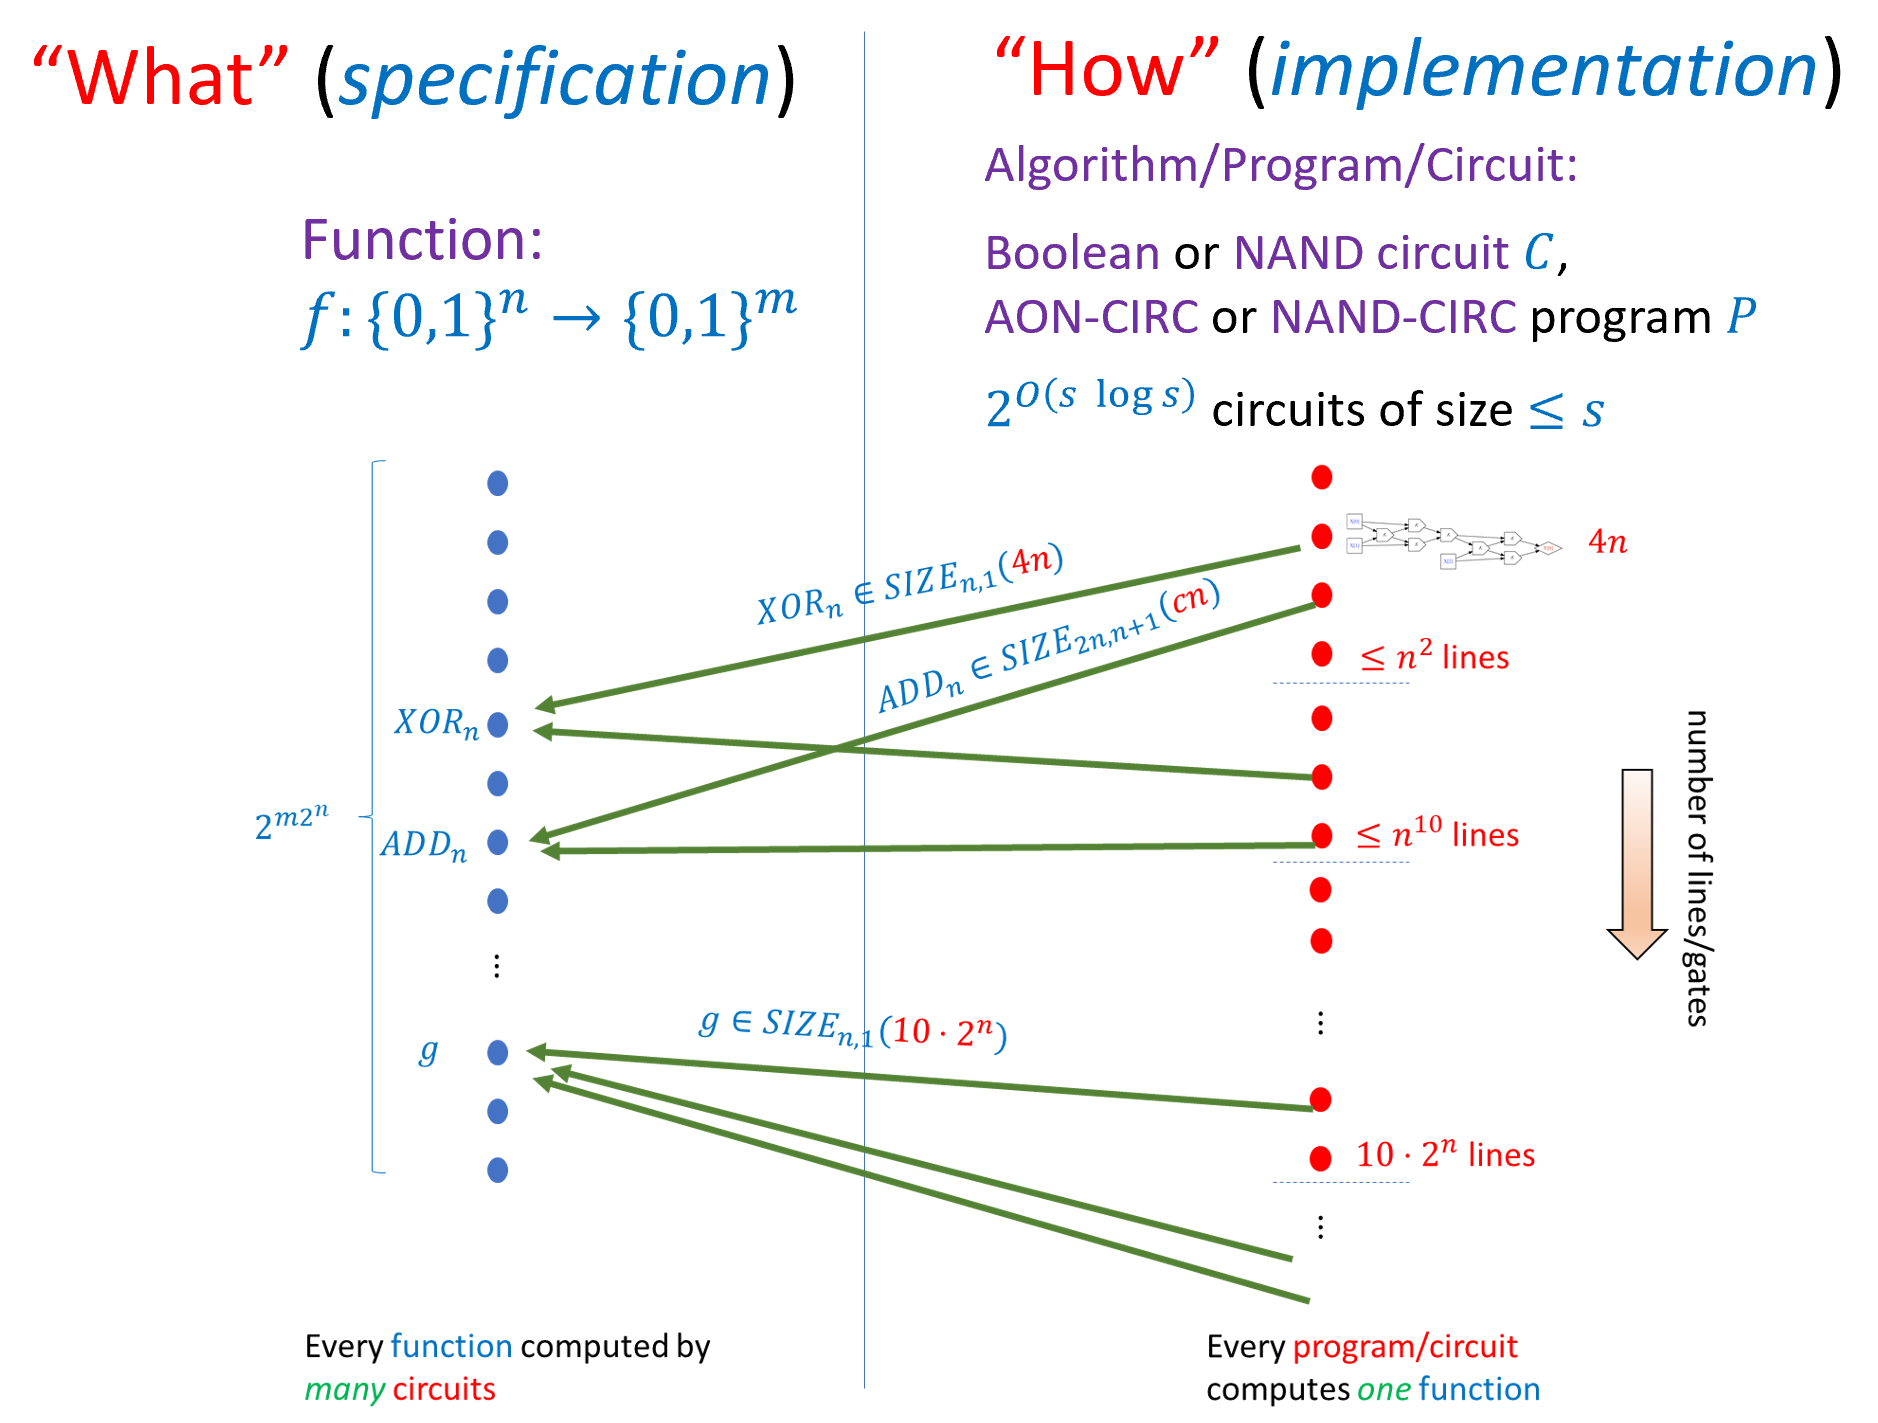
\includegraphics[width=\textwidth, height=0.25\paperheight, keepaspectratio]{../figure/finitecomprecap.png}
\caption{A finite computational task is specified by a function
\(f:\{0,1\}^n \rightarrow \{0,1\}^m\). We can model a computational
process using Boolean circuits (of varying gate sets) or straight-line
program. Every function can be computed by many programs. We say that
\(f \in \ensuremath{\mathit{SIZE}}_{n,m}(s)\) if there exists a NAND
circuit of at most \(s\) gates (equivalently a NAND-CIRC program of at
most \(s\) lines) that computes \(f\). Every function
\(f:\{0,1\}^n \rightarrow \{0,1\}^m\) can be computed by a circuit of
\(O(m \cdot 2^n/n)\) gates. Many functions such as multiplication,
addition, solving linear equations, computing the shortest path in a
graph, and others, can be computed by circuits of much fewer gates. In
particular there is an \(O(s^2 \log s)\)-size circuit that computes the
map \(C,x \mapsto C(x)\) where \(C\) is a string describing a circuit of
\(s\) gates. However, the counting argument shows there do exist some
functions \(f:\{0,1\}^n \rightarrow \{0,1\}^m\) that require
\(\Omega(m \cdot 2^n /n)\) gates to compute.}
\label{finiterecapfig}
\end{figure}

\section{Recap of Part I: Finite
Computation}\label{Recap-of-Part-I-Finite-Co}

This chapter concludes the first part of this book that deals with
\emph{finite computation} (computing functions that map a fixed number
of Boolean inputs to a fixed number of Boolean outputs). The main
take-aways from \cref{compchap}, \cref{finiteuniversalchap}, and
\cref{codeanddatachap} are as follows (see also \cref{finiterecapfig}):

\begin{itemize}
\item
  We can formally define the notion of a function
  \(f:\{0,1\}^n \rightarrow \{0,1\}^m\) being computable using \(s\)
  basic operations. Whether these operations are AND/OR/NOT, NAND, or
  some other universal basis does not make much difference. We can
  describe such a computation either using a \emph{circuit} or using a
  \emph{straight-line program}.
\item
  We define \(\ensuremath{\mathit{SIZE}}_{n,m}(s)\) to be the set of
  \emph{functions} that are computable by NAND circuits of at most \(s\)
  gates. This set is equal to the set of functions computable by a
  NAND-CIRC program of at most \(s\) lines and up to a constant factor
  in \(s\) (which we will not care about); this is also the same as the
  set of functions that are computable by a Boolean circuit of at most
  \(s\) AND/OR/NOT gates. The class
  \(\ensuremath{\mathit{SIZE}}_{n,m}(s)\) is a set of \emph{functions},
  not of programs/circuits.
\item
  \emph{Every} function \(f:\{0,1\}^n \rightarrow \{0,1\}^m\) can be
  computed using a circuit of \emph{at most} \(O(m \cdot 2^n / n)\)
  gates. \emph{Some} functions require \emph{at least}
  \(\Omega(m \cdot 2^n /n)\) gates. We define
  \(\ensuremath{\mathit{SIZE}}_{n,m}(s)\) to be the set of functions
  from \(\{0,1\}^n\) to \(\{0,1\}^m\) that can be computed using at most
  \(s\) gates.
\item
  We can describe a circuit/program \(P\) as a string. For every \(s\),
  there is a \emph{universal} circuit/program \(U_s\) that can evaluate
  programs of length \(s\) given their description as strings. We can
  use this representation also to \emph{count} the number of circuits of
  at most \(s\) gates and hence prove that some functions cannot be
  computed by circuits of smaller-than-exponential size.
\item
  If there is a circuit of \(s\) gates that computes a function \(f\),
  then we can build a physical device to compute \(f\) using \(s\) basic
  components (such as transistors). The ``Physical Extended
  Church-Turing Thesis'' postulates that the reverse direction is true
  as well: if \(f\) is a function for which \emph{every} circuit
  requires at least \(s\) gates then that \emph{every} physical device
  to compute \(f\) will require about \(s\) ``physical resources''. The
  main challenge to the PECTT is \emph{quantum computing}, which we will
  discuss in \cref{quantumchap}.
\end{itemize}

\paragraph{Sneak preview:} In the next part we will discuss how to model
computational tasks on \emph{unbounded inputs}, which are specified
using functions \(F:\{0,1\}^* \rightarrow \{0,1\}^*\) (or
\(F:\{0,1\}^* \rightarrow \{0,1\}\)) that can take an unbounded number
of Boolean inputs.

\section{Exercises}\label{Exercises}

\hypertarget{reading-comp}{}
\begin{exercise} \label[exercise]{reading-comp}

Which one of the following statements is false:

\begin{enumerate}
\def\labelenumi{\alph{enumi}.}
\item
  There is an \(O(s^3)\) line NAND-CIRC program that given as input
  program \(P\) of \(s\) lines in the list-of-tuples representation
  computes the output of \(P\) when all its input are equal to \(1\).
\item
  There is an \(O(s^3)\) line NAND-CIRC program that given as input
  program \(P\) of \(s\) characters encoded as a string of \(7s\) bits
  using the ASCII encoding, computes the output of \(P\) when all its
  input are equal to \(1\).
\item
  There is an \(O(\sqrt{s})\) line NAND-CIRC program that given as input
  program \(P\) of \(s\) lines in the list-of-tuples representation
  computes the output of \(P\) when all its input are equal to \(1\).
\end{enumerate}

\end{exercise}

\hypertarget{equals}{}
\begin{exercise}[Equals function] \label[exercise]{equals}

For every \(k \in \N\), show that there is an \(O(k)\) line NAND-CIRC
program that computes the function
\(\ensuremath{\mathit{EQUALS}}_k:\{0,1\}^{2k} \rightarrow \{0,1\}\)
where \(\ensuremath{\mathit{EQUALS}}(x,x')=1\) if and only if \(x=x'\).

\end{exercise}

\hypertarget{equalstwo}{}
\begin{exercise}[Equal to constant function] \label[exercise]{equalstwo}

For every \(k \in \N\) and \(x' \in \{0,1\}^k\), show that there is an
\(O(k)\) line NAND-CIRC program that computes the function
\(\ensuremath{\mathit{EQUALS}}_{x'} : \{0,1\}^k \rightarrow \{0,1\}\)
that on input \(x\in \{0,1\}^k\) outputs \(1\) if and only if \(x=x'\).

\end{exercise}

\hypertarget{countingmultibitex}{}
\begin{exercise}[Counting lower bound for multibit functions] \label[exercise]{countingmultibitex}

Prove that there exists a number \(\delta>0\) such that for every
\(n,m\) there exists a function \(f:\{0,1\}^n \rightarrow \{0,1\}^m\)
that requires at least \(\delta m \cdot 2^n / n\) NAND gates to compute.
See footnote for hint.\footnote{How many functions from \(\{0,1\}^n\) to
  \(\{0,1\}^m\) exist?}

\end{exercise}

\hypertarget{sizehiearchyex}{}
\begin{exercise}[Size hierarchy theorem for multibit functions] \label[exercise]{sizehiearchyex}

Prove that there exists a number \(C\) such that for every \(n,m\) and
\(n+m < s < m\cdot 2^n / (Cn)\) there exists a function
\(f \in \ensuremath{\mathit{SIZE}}_{n,m}(C\cdot s) \setminus \ensuremath{\mathit{SIZE}}_{n,m}(s)\).
See footnote for hint.\footnote{Follow the proof of
  \cref{sizehiearchythm}, replacing the use of the counting argument
  with \cref{countingmultibitex}.}

\end{exercise}

\hypertarget{efficientrepresentationex}{}
\begin{exercise}[Efficient representation of circuits and a tighter counting upper bound] \label[exercise]{efficientrepresentationex}

Use the ideas of \cref{efficientrepresentation} to show that for every
\(\epsilon>0\) and sufficiently large \(s,n,m\),
\[|\ensuremath{\mathit{SIZE}}_{n,m}(s)| < 2^{(2+\epsilon)s \log s + n\log n + m\log s}\;.\]
Conclude that the implicit constant in \cref{program-count} can be made
arbitrarily close to \(5\). See footnote for hint.\footnote{Using the
  adjacency list representation, a graph with \(n\) in-degree zero
  vertices and \(s\) in-degree two vertices can be represented using
  roughly \(2s\log(s+n) \leq 2s (\log s + O(1))\) bits. The labeling of
  the \(n\) input and \(m\) output vertices can be specified by a list
  of \(n\) labels in \([n]\) and \(m\) labels in \([m]\).}

\end{exercise}

\hypertarget{efficientlbex}{}
\begin{exercise}[Tighter counting lower bound] \label[exercise]{efficientlbex}

Prove that for every \(\delta< 1/2\), if \(n\) is sufficiently large
then there exists a function \(f:\{0,1\}^n \rightarrow \{0,1\}\) such
that
\(f \not\in \ensuremath{\mathit{SIZE}}_{n,1}\left( \tfrac{\delta 2^n}{n} \right)\).
See footnote for hint.\footnote{\emph{Hint:} Use the results of
  \cref{efficientrepresentationex} and the fact that in this regime
  \(m=1\) and \(n\ll s\).}

\end{exercise}

\hypertarget{rand-lb-id}{}
\begin{exercise}[Random functions are hard] \label[exercise]{rand-lb-id}

Suppose \(n>1000\) and that we choose a function
\(F:\{0,1\}^n \rightarrow \{0,1\}\) at random, choosing for every
\(x\in \{0,1\}^n\) the value \(F(x)\) to be the result of tossing an
independent unbiased coin. Prove that the probability that there is a
\(2^n/(1000n)\) line program that computes \(F\) is at most
\(2^{-100}\).\footnote{\textbf{Hint:} An equivalent way to say this is
  that you need to prove that the set of functions that can be computed
  using at most \(2^n/(1000n)\) lines has fewer than \(2^{-100}2^{2^n}\)
  elements. Can you see why?}

\end{exercise}

\begin{exercise} \label[exercise]{The-following-is-a-tuple-}

The following is a tuple representing a NAND program:
\((3, 1, ((3, 2, 2), (4, 1, 1), (5, 3, 4), (6, 2, 1), (7, 6, 6), (8, 0, 0), (9, 7, 8), (10, 5, 0), (11, 9, 10))\).

\begin{enumerate}
\def\labelenumi{\arabic{enumi}.}
\item
  Write a table with the eight values \(P(000)\), \(P(001)\),
  \(P(010)\), \(P(011)\), \(P(100)\), \(P(101)\), \(P(110)\), \(P(111)\)
  in this order.
\item
  Describe what the programs does in words.
\end{enumerate}

\end{exercise}

\hypertarget{XOREVAL}{}
\begin{exercise}[EVAL with XOR] \label[exercise]{XOREVAL}

For every sufficiently large \(n\), let
\(E_n:\{0,1\}^{n^2} \rightarrow \{0,1\}\) be the function that takes an
\(n^2\)-length string that encodes a pair \((P,x)\) where
\(x\in \{0,1\}^n\) and \(P\) is a NAND program of \(n\) inputs, a single
output, and at most \(n^{1.1}\) lines, and returns the output of \(P\)
on \(x\).\footnote{Note that if \(n\) is big enough, then it is easy to
  represent such a pair using \(n^2\) bits, since we can represent the
  program using \(O(n^{1.1}\log n)\) bits, and we can always pad our
  representation to have exactly \(n^2\) length.} That is,
\(E_n(P,x)=P(x)\).

Prove that for every sufficiently large \(n\), there \emph{does not
exist} an XOR circuit \(C\) that computes the function \(E_n\), where a
XOR circuit has the \(\ensuremath{\mathit{XOR}}\) gate as well as the
constants \(0\) and \(1\) (see \cref{xorex}). That is, prove that there
is some constant \(n_0\) such that for every \(n>n_0\) and XOR circuit
\(C\) of \(n^2\) inputs and a single output, there exists a pair
\((P,x)\) such that \(C(P,x) \neq E_n(P,x)\).

\end{exercise}

\hypertarget{learningcircuitsex}{}
\begin{exercise}[Learning circuits (challenge, optional, assumes more background)] \label[exercise]{learningcircuitsex}

(This exercise assumes background in probability theory and/or machine
learning that you might not have at this point. Feel free to come back
to it at a later point and in particular after going over
\cref{probabilitychap}.) In this exercise we will use our bound on the
number of circuits of size \(s\) to show that (if we ignore the cost of
computation) every such circuit can be \emph{learned} from not too many
training samples. Specifically, if we find a size-\(s\) circuit that
classifies correctly a training set of \(O(s \log s)\) samples from some
distribution \(D\), then it is guaranteed to do well on the whole
distribution \(D\). Since Boolean circuits model very many physical
processes (maybe even all of them, if the (controversial) physical
extended Church-Turing thesis is true), this shows that all such
processes could be learned as well (again, ignoring the computation cost
of finding a classifier that does well on the training data).

Let \(D\) be any probability distribution over \(\{0,1\}^n\) and let
\(C\) be a NAND circuit with \(n\) inputs, one output, and size
\(s \geq n\). Prove that there is some constant \(c\) such that with
probability at least \(0.999\) the following holds: if
\(m = c s \log s\) and \(x_0,\ldots,x_{m-1}\) are chosen independently
from \(D\), then for every circuit \(C'\) such that \(C'(x_i)=C(x_i)\)
on every \(i \in [m]\), \(\Pr_{x \sim D}[C'(x) \leq C(x)] \leq 0.99\).

In other words, if \(C'\) is a so called ``empirical risk minimizer''
that agrees with \(C\) on all the training examples
\(x_0,\ldots,x_{n-1}\), then it will also agree with \(C\) with high
probability for samples drawn from the distribution \(D\) (i.e., it
``generalizes'', to use Machine-Learning lingo). See footnote for
hint.\footnote{\emph{Hint:} Use our bound on the number of
  programs/circuits of size \(s\) (\cref{program-count}), as well as the
  Chernoff Bound ( \cref{chernoffthm}) and the union bound.}

\end{exercise}

\section{Bibliographical notes}\label{bibnotescodeasdata}

The \(\ensuremath{\mathit{EVAL}}\) function is usually known as a
\emph{universal circuit}. The implementation we describe is not the most
efficient known. Valiant \cite{Valiant1976} first showed a universal
circuit of \(O(n \log n)\) size where \(n\) is the size of the input.
Universal circuits have seen in recent years new motivations due to
their applications for cryptography, see
\cite{lipmaa2016valiant, Gunther2017} .

While we've seen that ``most'' functions mapping \(n\) bits to one bit
require circuits of exponential size \(\Omega(2^n/n)\), we actually do
not know of any \emph{explicit} function for which we can \emph{prove}
that it requires, say, at least \(n^{100}\) or even \(100n\) size. At
the moment, the strongest such lower bound we know is that there are
quite simple and explicit \(n\)-variable functions that require at least
\((5-o(1))n\) lines to compute, see
\href{http://www.wisdom.weizmann.ac.il/~ranraz/publications/P5nlb.pdf}{this
paper of Iwama et al} as well as this more recent
\href{http://logic.pdmi.ras.ru/~kulikov/papers/2012_5n_lower_bound_cie.pdf}{work
of Kulikov et al}. Proving lower bounds for restricted models of
circuits is an extremely interesting research area, for which Jukna's
book \cite{Jukna12} (see also Wegener \cite{wegener1987complexity})
provides a very good introduction and overview. I learned of the proof
of the size hierarchy theorem (\cref{sizehiearchythm}) from Sasha
Golovnev.

Scott Aaronson's blog post on how
\href{http://www.scottaaronson.com/blog/?p=3327}{information is
physical} is a good discussion on issues related to the physical
extended Church-Turing Physics. Aaronson's survey on NP complete
problems and physical reality \cite{aaronson2005physicalreality}
discusses these issues as well, though it might be easier to read after
we reach \cref{cooklevinchap} on \(\mathbf{NP}\) and
\(\mathbf{NP}\)-completeness.
